\documentclass[lettersize,journal]{IEEEtran}
\usepackage{amsmath,amsfonts}
\usepackage{algorithmic}
\usepackage{algorithm}
%\usepackage{algpseudocode}
\usepackage{float}
\usepackage{array}
\usepackage[caption=false,font=normalsize,labelfont=sf,textfont=sf]{subfig}
\usepackage{textcomp}
\usepackage{stfloats}
\usepackage{makecell}
\usepackage{multirow}
\usepackage{booktabs}
\usepackage{xcolor}
\newtheorem{theorem}{Theorem}
\newtheorem{corollary}{Corollary}
\usepackage{url}
\setlength{\textfloatsep}{8pt plus 2pt minus 2pt}   % 浮动体在页顶/页底时与正文距离
\setlength{\intextsep}{8pt plus 2pt minus 2pt}      % 浮动体插在正文中间时与正文距离
\setlength{\floatsep}{8pt plus 2pt minus 2pt}       % 两个浮动体之间距离
\setlength{\abovecaptionskip}{4pt}
\setlength{\belowcaptionskip}{0pt}
\newcommand{\vect}[1]{\boldsymbol{#1}}
\newcommand{\R}{\mathbb{R}}
\usepackage{amssymb,bm}
\usepackage{verbatim}
\usepackage{graphicx}
\usepackage{cite}
\hyphenation{op-tical net-works semi-conduc-tor IEEE-Xplore}
% updated with editorial comments 8/9/2021

\begin{document}

\title{Event-Triggered Nonlinear Model Predictive Control for Energy-Aware UAV Obstacle Avoidance}

\author{
	Heng Zhang, \IEEEmembership{Member, IEEE}, Liang Yuan, Xianghui Cao, \IEEEmembership{Senior Member, IEEE}
	\thanks{
		This work was supported in part by the National Natural Science Foundation of China under Grant 61873106,
		the Nature Science Foundation of Jiangsu Province for Distinguished Young Scholars under Grant BK20200049,
		and the Jiangsu Province Graduate Student Scientific Research Innovation Program under Grant SY202572X.
		(Corresponding author: Heng Zhang)
	}
	\thanks{
		Heng Zhang is with the College of Computer Engineering,
		Jiangsu Ocean University, Lianyungang 222005, China.
		(E-mail: ezhangheng@gmail.com).
	}
	\thanks{
		Liang Yuan is with the College of Electronic Engineering, Jiangsu Ocean University, Lianyungang 222005, China.
		(E-mail: yuanliang@jou.edu.cn).
	}
	\thanks{
		Xianghui Cao is with the School of Automation,
		Southeast University, Nanjing, 210096, China.
		(E-mail: xhcao@seu.edu.cn).
	}
}

% The paper headers
\markboth{Journal of \LaTeX\ Class Files,~Vol.~14, No.~8, August~2021}%
{Shell \MakeLowercase{\textit{et al.}}: A Sample Article Using IEEEtran.cls for IEEE Journals}

%\IEEEpubid{0000--0000/00\$00.00~\copyright~2021 IEEE}
% Remember, if you use this you must call \IEEEpubidadjcol in the second
% column for its text to clear the IEEEpubid mark.

\maketitle

\begin{abstract}
	This paper proposes an event-triggered dual-mode nonlinear model predictive control (NMPC) framework for autonomous obstacle avoidance of uncrewed aerial vehicles (UAVs) in complex 3D dynamic environments. \textcolor{blue}{The framework is positioned in an IoT-enabled cyber--physical system, where the UAV operates as a mobile sensing-and-actuation node that converts available obstacle observations into safety-critical motion decisions.} To balance \textcolor{blue}{computational efficiency and resource-aware computation reduction} with motion safety while considering \textcolor{blue}{the energy-related trade-off}, a composite risk assessment mechanism is developed to schedule the NMPC solver according to instantaneous collision threats. Under low-risk conditions, the UAV follows nominal trajectory tracking. Under high-risk conditions, local predictive replanning is activated to generate a safe avoidance trajectory. By integrating a Kalman-based predictive horizon, the framework enables the UAV to anticipate heterogeneous dynamic obstacle motions and proactively avoid potential conflicts. \textcolor{blue}{An asymmetric climb penalty is also introduced as an energy-aware altitude regulation mechanism that shapes the optimization preference for positive altitude gains.} Extensive simulations, profiling experiments, and Monte Carlo stress tests show that the proposed framework maintains a 100\% obstacle-avoidance success rate under measurement noise and increasing obstacle density. \textcolor{blue}{Compared with the continuous NMPC baseline, the proposed method reduces average CPU time by 21.1\%--24.2\% in the reported desktop MATLAB/CasADi profiling experiments while preserving reliable clearance and stable solver behavior.}
\end{abstract}

\begin{IEEEkeywords}
	Computational efficiency, event-triggered control, nonlinear model predictive control, obstacle avoidance, receding horizon prediction, uncrewed aerial vehicles.
\end{IEEEkeywords}

\section{Introduction}

Autonomous navigation in complex 3D environments remains a critical challenge for uncrewed aerial vehicles (UAVs) \cite{ref1}. In these environments, UAVs must respond quickly to obstacles and other changes. At the same time, they must limit energy consumption to maintain sufficient flight endurance \cite{ref2}. Therefore, the trajectory planning and control method must consider safety, maneuverability, and energy efficiency together. Nonlinear model predictive control (NMPC) is a promising solution for this problem. It can handle nonlinear system dynamics and operational constraints explicitly. It can also generate proactive maneuvers for obstacle avoidance \cite{ref3}. However, NMPC usually requires the controller to solve an optimization problem at every sampling instant. This process creates a heavy computational burden. As a result, real-time implementation becomes difficult on UAV flight controllers with limited onboard computing resources.

\textcolor{blue}{In an IoT-enabled cyber--physical system, the UAV can operate as a mobile sensing-and-actuation node that closes a local perception--decision--actuation loop: it uses environmental observations for local situation assessment, selects a control action, and executes the resulting maneuver.}

Accurate environmental representation is essential for safe online planning. Recent studies use continuous occupancy mapping \cite{ref4} and risk-aware spatio-temporal corridors \cite{ref5} to describe safe flight regions. Topological risk-based path selection \cite{ref6} and integrated cost assessment models \cite{ref7, ref8} further improve planning reliability in dense urban areas. These methods provide an important foundation for safe trajectory generation.
Based on these safety representations, predictive planning methods use motion forecasting \cite{ref9, ref10}, intent prediction \cite{ref11}, predictive velocity obstacles \cite{ref12, ref13}, and active perception-planning collaboration \cite{ref14} to detect future conflicts and improve navigation performance. In addition, reactive planning methods under limited sensing \cite{ref15, ref16} can improve decision-making in dynamic environments. However, the computational cost of predictive planning increases as the number of obstacles grows and the prediction horizon becomes longer.

To reduce the computational cost of predictive planning, recent studies have introduced event-triggered (ET) control as an efficient solution. ET control has been applied in networked systems \cite{ref17, ref18}, adaptive control \cite{ref19, ref20, ref21}, and predictive control for several platforms \cite{ref22, ref23, ref24, ref25}. These studies show that ET control can improve computational efficiency. However, existing ET-NMPC methods still do not fully consider obstacle motion trends or real-time collision risk. As a result, delayed responses may occur in high-speed 3D obstacle avoidance tasks.

The UAV obstacle avoidance also depends on energy efficiency because onboard battery capacity is limited. Recent studies have used propulsion models \cite{ref26, ref27, ref28} for energy-aware optimization in Internet of Things (IoT) networks \cite{ref29, ref30}. Some methods further apply reinforcement learning \cite{ref31} and resource allocation \cite{ref32} to improve energy performance. However, many of these methods focus on communication tasks and assume static environments \cite{ref33}. Therefore, they are not well suited for dynamic obstacle avoidance under uncertainty.

\textcolor{blue}{Within this context, the present work focuses on the local perception--control computation required for dynamic obstacle avoidance. It does not model communication scheduling, radio resource allocation, or communication-energy optimization; these aspects are outside the scope of the proposed control formulation.}

In complex 3D navigation, UAVs require on-demand solver activation, risk-aware threat assessment, and energy-aware maneuver regulation. However, existing methods rarely integrate these requirements into a unified obstacle-avoidance framework. To address this limitation, we propose an energy-aware ET-NMPC framework for 3D dynamic environments. The framework combines a risk-triggered dual-mode mechanism, a composite risk index, and an asymmetric energy penalty. \textcolor{blue}{These designs reduce unnecessary NMPC calls, schedule replanning according to real-time collision risk, and introduce energy-aware altitude regulation that shapes the optimization preference for positive altitude gains.}

\textcolor{blue}{The event-triggered mechanism reduces unnecessary optimization activations and computational workload, while the current study focuses on desktop MATLAB/CasADi computational characterization rather than strict onboard real-time validation. Accordingly, the reported CPU-time reductions represent relative computational savings, not a hard real-time guarantee.}

\textcolor{blue}{From an IoT-system perspective, the event-triggered mechanism performs resource-aware local decision scheduling by avoiding unnecessary NMPC solver activations and reducing the associated local controller-computation workload.}

The main contributions of this work are summarized as follows:
\begin{itemize}
	\item A risk-triggered dual-mode NMPC mechanism is developed to switch between lightweight nominal tracking and local predictive replanning. This mechanism activates the NMPC solver only in high-risk situations and reduces unnecessary optimization calls.
	
	\item A composite risk index is designed by integrating encounter risk, predictive occupancy risk, and reference deviation risk. This index enables the controller to evaluate dynamic collision threats and schedule replanning according to real-time risk.
	
	\item \textcolor{blue}{An energy-aware NMPC cost with an asymmetric climb penalty is introduced for 3D UAV obstacle avoidance. The additional penalty on positive altitude gains provides energy-aware altitude regulation by shaping the optimization preference among altitude motion, safety, and energy-related cost.}
\end{itemize}

The remainder of this paper is organized as follows. Section II presents system modeling. Section III describes the ET-NMPC framework. Section IV gives simulation results, and Section V concludes the paper.

For readability, the main abbreviations used in this paper are summarized in Table~\ref{tab:abbreviations}.

\begin{table}[t]
	\centering
	\caption{List of Abbreviations}
	\label{tab:abbreviations}
	\footnotesize
	\renewcommand{\arraystretch}{1.12}
	\begin{tabular}{@{} p{0.28\columnwidth} p{0.62\columnwidth} @{}}
		\toprule
		\textbf{Abbreviation} & \textbf{Full Name} \\
		\midrule
		UAV & Uncrewed Aerial Vehicle \\
		IoT & Internet of Things \\
		CPU & Central Processing Unit \\
		MPC & Model Predictive Control \\
		NMPC & Nonlinear Model Predictive Control \\
		ET & Event-Triggered \\
		ET-NMPC & Event-Triggered Nonlinear Model Predictive Control \\
		C-NMPC & Continuous Nonlinear Model Predictive Control \\
		NP-ET-NMPC & Event-Triggered NMPC without Prediction \\
		SE-ET-NMPC & Event-Triggered NMPC with Symmetric Energy Cost \\
		TCPA & Time to Closest Point of Approach \\
		DCPA & Distance at Closest Point of Approach \\
		CV & Constant Velocity \\
		CA & Constant Acceleration \\
		SIN & Sinusoidal Motion \\
		RAND & Random Maneuvering Motion \\
		NLP & Nonlinear Programming \\
		IPOPT & Interior Point Optimizer \\
		APF & Artificial Potential Field \\
		3D-APF & Three-Dimensional Artificial Potential Field \\
		RRT$^\ast$ & Rapidly-Exploring Random Tree Star \\
		\bottomrule
	\end{tabular}
\end{table}

\section{SYSTEM MODELING}

This section addresses the online obstacle-avoidance problem for a UAV in 3D environments with static and dynamic obstacles. As illustrated in Fig. 1, the vehicle must reach a target while satisfying velocity, control, and altitude constraints under environmental uncertainty. We establish the workspace, kinematic, and obstacle models to support the subsequent event-triggered planning framework.

\textcolor{blue}{The UAV is modeled as a mobile sensing-and-actuation node in an IoT-enabled cyber--physical system. At each sampling instant, the local perception--decision--actuation loop processes available obstacle observations, predicts their future motion, assesses collision risk, selects an operating mode, and applies the corresponding control action. This work models this local loop and its motion consequences.}

\begin{figure}[h!]
	\centering
	\includegraphics[width=3.2in]{1}
	\caption{Illustration of the 3D workspace, UAV state variables, and obstacle models. The UAV starts from $\vect{p}_s$ and moves toward the target $\vect{p}_g$ while satisfying velocity, acceleration, altitude, and safety-radius constraints. Static obstacles are represented by $\mathcal{O}_s$, and dynamic obstacles are described by their positions, velocities, and spherical safety regions.}
	\vspace{-6pt}
\end{figure}


\subsection{Workspace and UAV Kinematics}

The UAV operates within a bounded three-dimensional workspace $\mathcal{W} \subset \mathbb{R}^{3}$, where $\mathcal{W}$ denotes the admissible flight region. The UAV initiates its mission from a starting position $\vect{p}_s \in \mathcal{W}$ with the objective of reaching a target $\vect{p}_g \in \mathcal{W}$. For collision avoidance modeling, the UAV is approximated as a sphere with a safety radius $r_u > 0$. Static obstacles, such as buildings and fixed facilities, are characterized by the closed set $\mathcal{O}_s \subset \mathcal{W}$.


To balance model fidelity with online computational efficiency, the UAV state \cite{ref3} at time step $k$ is defined as $\vect{x}_k = [\vect{p}_k^\top, \vect{v}_k^\top]^\top \in \mathbb{R}^{6}$, where $\vect{p}_k = [x_k, y_k, z_k]^\top \in \mathbb{R}^3$ and $\vect{v}_k = [v_{x,k}, v_{y,k}, v_{z,k}]^\top \in \mathbb{R}^3$ denote the position and velocity vectors, respectively. The UAV dynamics are governed by the following discrete-time kinematic equations
\begin{align}
	\vect{p}_{k+1} &= \vect{p}_k + \vect{v}_k \Delta t, \label{eq:pk} \\
	\vect{v}_{k+1} &= \vect{v}_k + \vect{u}_k \Delta t, \label{eq:vk}
\end{align}
where $\vect{u}_k \in \mathbb{R}^{3}$ is the control input representing commanded acceleration. The flight envelope is subject to the following hard constraints
\begin{equation}
	\|\vect{v}_k\| \le v_{\max}, \quad \|\vect{u}_k\| \le u_{\max}, \quad z_{\min} \le z_k \le z_{\max},
	\label{eq:uav_constraints}
\end{equation}
where $v_{\max}$ and $u_{\max}$ are the maximum allowable speed and acceleration magnitude. In addition to the overall speed bound, the vertical maneuver is further limited by $|v_{z,k}| \le v_{z,\max}$ to reflect the asymmetric climb capability of the UAV. Based on these kinematic foundations, the obstacle observation process is introduced next for risk-aware online planning.

\subsection{Dynamic Obstacle Observation Model}

In an environment with $N_o$ dynamic obstacles, the state of the $i$-th obstacle at time step $k$ is defined as $\vect{o}_i(k) = [\vect{\xi}_i(k)^\top, \vect{\zeta}_i(k)^\top]^\top$. Here, $\vect{\xi}_i(k) \in \mathbb{R}^3$ represents the 3D position vector. $\vect{\zeta}_i(k) \in \mathbb{R}^3$ represents the 3D velocity vector. Each obstacle is modeled as a sphere with radius $r_i$. For online prediction, obstacles follow a discrete-time constant-velocity (CV) model \cite{ref9}
\begin{equation}
	\vect{o}_i(k+1) = \vect{A} \vect{o}_i(k) + \vect{w}_i(k),
	\label{eq:obs_dynamics}
\end{equation}
where $\vect{A}$ is the state transition matrix. $\vect{w}_i(k) \sim \mathcal{N}(\vect{0}, \vect{Q}_i)$ is the process noise. The observation model is formulated as
\begin{equation}
	\vect{y}_i(k) = \vect{C} \vect{o}_i(k) + \vect{n}_i(k),
	\label{eq:obs_measurement}
\end{equation}
where $\vect{y}_i(k) \in \mathbb{R}^3$ is the position measurement. $\vect{n}_i(k) \sim \mathcal{N}(\vect{0}, \vect{R}_i)$ is the measurement noise. Matrix $\vect{C}$ extracts the position component $\vect{\xi}_i(k)$ from the state vector. 

\textcolor{blue}{Here, $\vect{y}_i(k)$ represents the available obstacle observation provided to the local perception--control loop at time step $k$.}

For obstacles with nonlinear or uncertain motion, extended Kalman filters or local linearization can be applied. In this work, the CV model is used as a lightweight online predictor for computational efficiency. In the experiments, the actual obstacle motions also include constant-acceleration, sinusoidal, and random maneuvering cases. These cases introduce model mismatch and are used to test robustness under more unpredictable conditions.

\section{Energy-Aware Event-Triggered NMPC Framework} 

The proposed ET-NMPC framework consists of obstacle prediction, composite risk assessment, event-triggered mode switching, local predictive optimization, and receding-horizon execution. The framework activates the NMPC solver only when the predicted collision risk exceeds a prescribed threshold.

\subsection{Overall Architecture}

The framework follows a closed-loop pipeline. At each sampling instant, the UAV updates obstacle observations, predicts future obstacle motion, evaluates the composite risk index, and determines the control mode. Under low-risk conditions, the UAV tracks the nominal reference trajectory, while under high-risk conditions the local NMPC solver generates a collision-free trajectory segment.

\textcolor{blue}{This dual-mode design enables risk-dependent switching between lightweight tracking and predictive replanning according to the estimated collision risk.}

\subsection{Spatiotemporal Prediction of Dynamic Obstacles}

A Kalman filter is used for online state estimation and multi-step prediction. For the $i$-th obstacle, the one-step prediction equations are
\begin{equation}
	\hat{\vect{o}}_i(k+1|k) = \vect{A}\hat{\vect{o}}_i(k|k),
\end{equation}
\begin{equation}
	\vect{P}_i(k+1|k) = \vect{A}\vect{P}_i(k|k)\vect{A}^{\top} + \vect{Q}_i,
\end{equation}
where $\hat{\vect{o}}_i(k|k)$ is the posterior state estimate. $\vect{P}_i(k|k)$ is the error covariance at step $k$. The corresponding $\tau$-step-ahead prediction is calculated as
\begin{equation}
	\hat{\vect{o}}_i(k+\tau|k) = \vect{A}^{\tau}\hat{\vect{o}}_i(k|k),
\end{equation}
\begin{equation}
	\vect{P}_i(k+\tau|k) = \vect{A}^{\tau}\vect{P}_i(k|k)(\vect{A}^{\tau})^{\top}
	+ \sum_{j=0}^{\tau-1}\vect{A}^{j}\vect{Q}_i(\vect{A}^{j})^{\top},
\end{equation}
where $\tau \in \{1, \ldots, H\}$ and $H$ is the prediction horizon.

Let $\vect{P}_{pos,i}(k+\tau|k) \in \R^{3\times 3}$ be the position covariance submatrix extracted from $\vect{P}_i(k+\tau|k)$. The 3D position error confidence ellipsoid is defined as
\begin{equation}
	\mathcal{E}_i(k+\tau|k) = \left\{ \vect{e} \in \R^3 : \vect{e}^{\top}\vect{P}_{pos,i}^{-1}(k+\tau|k)\vect{e} \le \chi_{3,\alpha}^{2} \right\}, \label{eq:error_ellipsoid}
\end{equation}
where $\chi_{3,\alpha}^{2}$ is the chi-square quantile with three degrees of freedom. This value is determined by the confidence level $\alpha$. 

A conservative spherical approximation is adopted to reduce computational cost. The uncertainty inflation radius \cite{ref5} is defined as
\begin{equation}
	\Delta_i(k+\tau) = \sqrt{\chi_{3,\alpha}^{2} \lambda_{\max}(\vect{P}_{pos,i}(k+\tau|k))}, 
\end{equation}
where $\lambda_{\max}(\cdot)$ denotes the maximum eigenvalue. The resulting spatiotemporal occupancy region $\mathcal{O}_i(k+\tau)$ \cite{ref5} is
\begin{equation}
	\small
	\mathcal{O}_i(k+\tau) = \{ \vect{p} \in \R^{3} : \|\vect{p} - \hat{\vect{\xi}}_i(k+\tau|k)\| \le r_i + \Delta_i(k+\tau) \}, 
\end{equation}
where $\hat{\vect{\xi}}_i(k+\tau|k)$ is the predicted position of the $i$-th obstacle. $r_i$ is its physical radius. The union of all occupancy regions is $\mathcal{O}(k+\tau) = \bigcup_{i=1}^{N_o} \mathcal{O}_i(k+\tau)$.

\subsection{Composite Risk Assessment and Event-Triggering Strategy}

After predicting obstacle motion, a composite risk index $R_k$ is built to quantify immediate threats. For the $i$-th obstacle, the relative position is $\vect{p}_{rel,i}(k) = \vect{p}_k - \vect{\xi}_i(k)$. The relative velocity is $\vect{v}_{rel,i}(k) = \vect{v}_k - \vect{\zeta}_i(k)$. 

Two key metrics assess the collision threat. $TCPA_i$ represents the Time to Closest Point of Approach and $DCPA_i$ represents the Distance at Closest Point of Approach. These metrics are calculated as
\begin{equation}
	TCPA_i(k) = -\frac{\vect{p}_{rel,i}^{\top}(k)\vect{v}_{rel,i}(k)}{\|\vect{v}_{rel,i}(k)\|^2+\varepsilon},
	\label{eq:tcpa}
\end{equation}
\begin{equation}
	DCPA_i(k) = \|\vect{p}_{rel,i}(k)+TCPA_i(k)\vect{v}_{rel,i}(k)\|,
	\label{eq:dcpa}
\end{equation}
where $\varepsilon > 0$ prevents division by zero. The encounter risk $\tilde{R}_k$ is defined as
\begin{equation}
	\tilde{R}_k = \max_i \left[ \exp \left( \frac{-TCPA_i^{+}}{T_c} \right) \exp \left( \frac{-DCPA_i}{D_c} \right) \right],
	\label{eq:rtcpa}
\end{equation}
where $TCPA_i^{+} = \max(TCPA_i,0)$, and $T_c, D_c$ are normalization constants.

The predictive risk $\hat{R}_k$ evaluates the proximity of the reference path to future occupancy regions
\begin{equation}
	\hat{R}_k = \max_{\tau, i} \frac{\rho_i(k+\tau)}{\|\vect{r}_{k+\tau}-\hat{\vect{\xi}}_i(k+\tau|k)\|+\varepsilon},
	\label{eq:rpred}
\end{equation}
\begin{equation}
	\rho_i(k+\tau) = r_u+r_i+\Delta_i(k+\tau)+d_m,
	\label{eq:rho}
\end{equation}
where $\vect{r}_{k+\tau}$ is the reference position at step $k+\tau$. $r_u$ and $d_m$ are safety radii. The deviation risk $\bar{R}_k$ penalizes tracking errors $\vect{e}_k = \vect{p}_k - \vect{r}_k$ and is defined as $\bar{R}_k = \|\vect{e}_k\| / (e_{\max} + \varepsilon)$. These terms are fused into the composite risk: $R_k = w_1 \tilde{R}_k + w_2 \hat{R}_k + w_3 \bar{R}_k$. Here, the weights satisfy $\sum w_i = 1$.

The switching logic with hysteresis and refractory protection is
\begin{equation}
	\sigma_k=
	\begin{cases}
		1, & R_k \ge R_{on} \text{ and } k - k_{last} \ge T_{ref},\\
		0, & R_k \le R_{off},\\
		\sigma_{k-1}, & \text{otherwise},
	\end{cases}
	\label{eq:trigger}
\end{equation}
where $R_{on}$ is the activation threshold and $R_{off}$ is the deactivation threshold. These values satisfy $R_{on} > R_{off}$. $T_{ref}$ is the refractory interval to prevent mode chattering. $k_{last}$ represents the time step of the most recent activation, which is reset to $k$ whenever $\sigma_k = 1$.

\subsection{Local Predictive Optimization Formulation}

When $\sigma_k=1$, the system constructs a finite-horizon local predictive optimization problem to generate a safe and dynamically feasible avoidance trajectory. The decision variables for this problem consist of the future position sequence $\Pi_k = \{\vect{p}_{k+1}, \vect{p}_{k+2}, \ldots, \vect{p}_{k+H}\}$ and the control-input sequence $U_k = \{\vect{u}_k, \vect{u}_{k+1}, \ldots, \vect{u}_{k+H-1}\}$, where $H$ denotes the prediction horizon.

\textcolor{blue}{To balance local-reference tracking, control regularization, energy awareness, and differentiable soft collision avoidance, the overall objective function $J$ is defined as}
\begin{equation}
	\small
	\textcolor{blue}{J = \rho_1 J_{\text{track}} + \rho_2 J_{\text{smooth}} + \rho_3 J_{\text{energy}} + \rho_4 J_{\text{risk}} + \rho_5 J_{\text{terminal}},}
	\label{eq:total_cost}
\end{equation}
\textcolor{blue}{where $J_{\text{track}}$, $J_{\text{smooth}}$, $J_{\text{energy}}$, $J_{\text{risk}}$, and $J_{\text{terminal}}$ denote the reference-tracking, control-increment, energy-aware, soft collision-avoidance, and terminal costs, respectively; $\rho_1,\ldots,\rho_5$ are their nonnegative weights. The risk-fusion weights $w_1,w_2,w_3$ retain their distinct meaning in Section~III-B.}

\textcolor{blue}{The reference-tracking cost is defined as}
\begin{equation}
	\textcolor{blue}{J_{\text{track}} = \sum_{\tau=0}^{H-1} \left\|\vect{p}_{k+\tau+1} - \vect{r}_{k+\tau+1}\right\|_2^2,}
	\label{eq:jtrack}
\end{equation}
\textcolor{blue}{where $\vect{r}_{k+\tau+1}$ is the local reference position at the corresponding prediction step. This term ensures that the UAV tracks the local reference trajectory during optimization. The control-increment penalty is defined as}
\begin{equation}
	\textcolor{blue}{J_{\text{smooth}} = \sum_{\tau=0}^{H-2} \left\|\vect{u}_{k+\tau+1} - \vect{u}_{k+\tau}\right\|_2^2,}
	\label{eq:jsmooth}
\end{equation}
\textcolor{blue}{which penalizes large variations in the predicted control sequence to improve trajectory executability.}

\textcolor{blue}{To implement energy-aware altitude regulation in the local optimization, the energy-aware cost $J_{energy}$ is defined as}
\begin{equation}
	\small
	\begin{aligned}
		\textcolor{blue}{J_{energy}}
		&= \textcolor{blue}{c_1 \sum_{\tau=0}^{H-1} \| \vect{p}_{k+\tau+1} - \vect{p}_{k+\tau} \|_2^2 + c_2 \sum_{\tau=0}^{H-1} \| \vect{u}_{k+\tau} \|_2^2} \\
		&\quad \textcolor{blue}{+ c_3 \sum_{\tau=0}^{H-1} \phi_{\epsilon}\!\left(z_{k+\tau+1} - z_{k+\tau}\right),}
	\end{aligned}
	\label{eq:jenergy}
\end{equation}
\textcolor{blue}{Here, $\phi_{\epsilon}(s)=\frac{1}{2}\left(s+\sqrt{s^2+\epsilon}\right)$ is a differentiable smooth approximation of the positive part of $s$, where $\epsilon>0$. The non-negative coefficients $c_1$, $c_2$, and $c_3$ weight the squared displacement, control-effort, and additional positive-altitude-gain terms, respectively. The third term assigns extra cost to positive altitude increments and therefore shapes the altitude-related optimization preference; it provides energy-aware altitude regulation rather than a guarantee of statistically significant mission-energy reduction. Thus, $J_{energy}$ remains a lightweight surrogate for online NMPC rather than a full rotor-level power model.}

\textcolor{blue}{To provide a quantitative model-based energy proxy beyond geometric metrics, the estimated energy is computed using a simplified physical model}
\begin{equation}
	E_{est}=P_{base}T+\frac{m g \Delta z_+}{\eta_c}+k_u\int_0^T \|u(t)\|^2 dt,
	\label{eq:estimated_energy}
\end{equation}
where $P_{base}$ is the baseline propulsion power, $T$ is the flight duration, $m$ is the UAV mass, $g$ is the gravitational acceleration, $\Delta z_+$ denotes the accumulated positive altitude change, $\eta_c$ is the climb efficiency, and $k_u$ is the maneuvering-energy coefficient. The three terms represent the baseline flight energy, climb-related potential energy, and additional energy caused by control effort, respectively. The estimated energy is converted into Watt-hours as $E_{Wh}=E_{est}/3600$. \textcolor{blue}{This quantity is a model-based mission-energy proxy for comparative analysis, rather than a hardware battery measurement, a power measurement, or a flight-energy validation result.}

\textcolor{blue}{The risk cost $J_{risk}$ is formulated as a differentiable soft collision-avoidance penalty over the predicted UAV--obstacle separations:}
\begin{equation}
	\begin{aligned}
		\textcolor{blue}{J_{\text{risk}}} &\textcolor{blue}{= \sum_{\tau=1}^{H} \Biggl(\sum_{i=1}^{N_o} \ell_{\mathrm{dyn}}\!\left(\left\|\vect{p}_{k+\tau}-\hat{\vect{\xi}}_i(k+\tau|k)\right\|_2,d^{\mathrm{safe}}_i(k+\tau)\right)} \\
		&\textcolor{blue}{\quad + \sum_{j=1}^{N_s} \ell_{\mathrm{stat}}\!\left(\vect{p}_{k+\tau},\mathcal{O}_j\right)\Biggr),}
	\end{aligned}
	\label{eq:jrisk}
\end{equation}
\textcolor{blue}{where $N_o$ and $N_s$ are the numbers of dynamic and static obstacles, respectively; $\mathcal{O}_j$ denotes the geometry of the $j$th static obstacle; and $d^{\mathrm{safe}}_i(k+\tau)$ is the safety radius of the $i$th dynamic obstacle. In this local optimization formulation, $d^{\mathrm{safe}}_i(k+\tau)=r_u+r_i+\Delta_i(k+\tau)+d_m$, which avoids overloading the objective-weight notation $\rho_1,\ldots,\rho_5$.}

\textcolor{blue}{The CasADi implementation uses the differentiable smooth positive operator}
\begin{equation*}
	\textcolor{blue}{[s]_{\epsilon}^{+}=\frac{1}{2}\left(s+\sqrt{s^2+\epsilon^2}\right),\qquad \epsilon>0.}
\end{equation*}
\textcolor{blue}{With $d$ denoting a predicted UAV--dynamic-obstacle distance, the dynamic penalty is}
\begin{equation*}
	\begin{aligned}
		\textcolor{blue}{\ell_{\mathrm{dyn}}\!\left(d,d^{\mathrm{safe}}\right)} &\textcolor{blue}{=g_{\mathrm{dyn}}\Bigl(\left[d^{\mathrm{safe}}-d\right]_{\epsilon}^{+}\Bigr)^3} \\
		&\textcolor{blue}{\quad+g_{\mathrm{near}}\Bigl(\left[d^{\mathrm{safe}}+b_{\mathrm{dyn}}-d\right]_{\epsilon}^{+}\Bigr)^2,}
	\end{aligned}
\end{equation*}
\textcolor{blue}{where $g_{\mathrm{dyn}}$, $g_{\mathrm{near}}$, and $b_{\mathrm{dyn}}$ are the dynamic-risk gain, near-obstacle gain, and near-obstacle buffer, respectively. For a static obstacle, the code uses the corresponding geometry-dependent smooth polynomial penalty}
\begin{equation*}
	\begin{aligned}
		\textcolor{blue}{\ell_{\mathrm{stat}}\!\left(\vect{p},\mathcal{O}_j\right)} &\textcolor{blue}{=q_j(\vect{p})g_{\mathrm{stat}}} \\
		&\textcolor{blue}{\quad\times\Bigl(\left[d^{\mathrm{safe}}_j-d_j\!\left(\vect{p},\mathcal{O}_j\right)\right]_{\epsilon}^{+}\Bigr)^4} \\
		&\textcolor{blue}{\quad+q_j(\vect{p})g_{\mathrm{stat,near}}} \\
		&\textcolor{blue}{\quad\times\Bigl(\left[d^{\mathrm{safe}}_j+b_{\mathrm{stat}}-d_j\!\left(\vect{p},\mathcal{O}_j\right)\right]_{\epsilon}^{+}\Bigr)^2} \\
		&\textcolor{blue}{\quad+q_j(\vect{p})g_{\mathrm{climb}}h_j(\vect{p})} \\
		&\textcolor{blue}{\quad\times\Bigl(\left[d^{\mathrm{safe}}_j+b_{\mathrm{stat}}-d_j\!\left(\vect{p},\mathcal{O}_j\right)\right]_{\epsilon}^{+}\Bigr)^2,}
	\end{aligned}
\end{equation*}
\textcolor{blue}{where $d_j(\vect{p},\mathcal{O}_j)$ is the geometry-dependent static-obstacle distance. The functions $q_j(\vect{p})$ and $h_j(\vect{p})$ denote the roof/altitude and climb-assistance factors, respectively. Thus, both obstacle terms are differentiable soft penalties rather than inverse-distance penalties.}

\textcolor{blue}{To explicitly account for terminal-goal attainment and progressively stronger attraction over the prediction horizon, the terminal cost is defined as}
\begin{equation}
	\begin{aligned}
		\textcolor{blue}{J_{\text{terminal}}} &\textcolor{blue}{=\lambda_p\left\|\vect{p}_{k+H}-\vect{p}_{\text{terminal\_ref}}\right\|_2^2+\lambda_v\left\|\vect{v}_{k+H}\right\|_2^2} \\
		&\textcolor{blue}{\quad+\lambda_{\text{prog}}\sum_{\tau=0}^{H-1}\left(\frac{\tau+1}{H}\right)^2\left\|\vect{p}_{k+\tau+1}-\vect{p}_{\text{terminal\_ref}}\right\|_2^2,}
	\end{aligned}
	\label{eq:jterminal}
\end{equation}
\textcolor{blue}{where the first two terms penalize terminal position error and terminal velocity, respectively. The final term is a stage-wise terminal-attraction penalty whose influence increases over the horizon. The terminal reference is $\vect{p}_{\text{goal}}$ when $\left\|\vect{p}_{k}-\vect{p}_{\text{goal}}\right\|_2\leq25\,\mathrm{m}$; otherwise, it is the last local reference point. Minimizing $J_{\text{terminal}}$ therefore promotes terminal convergence while avoiding residual terminal motion.}

This formulation enables the UAV to track a reference trajectory $\vect{r}_k$ while autonomously avoiding dynamic threats. Unlike conventional continuous schemes, we employ an on-demand strategy where the predictive optimizer is activated only when the instantaneous collision risk exceeds a prescribed threshold. Based on the estimated states $\hat{\vect{\xi}}_i(k)$, the goal is to compute an optimal control sequence that minimizes $J$ while maintaining safety and kinematic feasibility.

The resulting local predictive optimization problem is formulated as
\begin{subequations} 
	\label{eq:opt_problem}
	\begin{align}
		\min_{\Pi_k, U_k} \quad & J 
		\label{eq:obj} \\
		\text{s.t.} \quad 
		& \vect{p}_{k+\tau} = \vect{p}_{k+\tau-1} 
		+ \vect{v}_{k+\tau-1}\Delta t, 
		\label{eq:dyn1} \\
		& \vect{v}_{k+\tau} = \vect{v}_{k+\tau-1} 
		+ \vect{u}_{k+\tau-1}\Delta t, 
		\label{eq:dyn2} \\
		& \|\vect{u}_{k+\tau-1}\| \le u_{\max}, 
		\label{eq:constr_u} \\
		& \|\vect{v}_{k+\tau}\| \le v_{\max}, 
		\label{eq:constr_v} \\
		& z_{\min} \le z_{k+\tau} \le z_{\max}, 
		\label{eq:constr_z} \\
		& \|\vect{p}_{k+\tau} - \hat{\vect{\xi}}_i(k+\tau|k)\| 
		\ge d_{i,\tau}, 
		\label{eq:constr_dynobs} \\
		& \vect{p}_{k+\tau} \in \mathcal{W} \setminus \mathcal{O}_s.
		\label{eq:constr_staticobs}
	\end{align}
\end{subequations}
where $\Delta t$ is the sampling interval. The constraints are enforced for $\tau=1,\ldots,H$, and the dynamic obstacle constraint \eqref{eq:constr_dynobs} is further imposed for each obstacle $i=1,\ldots,N_o$. In \eqref{eq:constr_dynobs}, $d_{i,\tau}=r_u+r_i+\Delta_i(k+\tau)+d_m$ is the time-varying safety margin. Here, $d_m$ is a fixed minimum additional safety distance, whereas $d_{i,\tau}$ varies with the obstacle index, prediction step, and uncertainty inflation radius.

\subsection{Theoretical Analysis and Feasibility Discussion}

\textcolor{blue}{This section provides theoretical analysis for the proposed event-triggered dual-mode NMPC framework. The analysis first proves that the triggering mechanism excludes Zeno-like mode chattering. It then characterizes the computational complexity of prediction and event-triggered solver activation. Finally, recursive feasibility and closed-loop stability are discussed under bounded prediction errors and feasible replanning conditions.}

\begin{theorem}
	Consider the dual-mode switching logic defined in \eqref{eq:trigger}. For any sequence of triggering instants $\{k_1, k_2, \dots, k_j\}$, the number of sampling steps between any two consecutive activations $(\sigma_k = 1)$ is lower-bounded by $T_{ref}$
	\begin{equation}
		k_j - k_{j-1} \ge T_{ref}, \quad \forall j \in \mathbb{N}^{+}.
		\label{eq:theorem1_result}
	\end{equation}
\end{theorem}

\textit{Proof:} Let $k_{j-1}$ denote the time step of the $(j-1)$-th activation. According to the update rule, the auxiliary variable $k_{last}$ is reset to the current step at this instant
\begin{equation}
	k_{last} = k_{j-1}.
\end{equation}

According to the triggering condition in \eqref{eq:trigger}, the next activation at step $k_j$ occurs only if the refractory constraint is satisfied
\begin{equation}
	k_j - k_{last} \ge T_{ref}.
\end{equation}

Substituting the value of $k_{last}$ into the inequality yields
\begin{equation}
	k_j - k_{j-1} \ge T_{ref}.
\end{equation}

Define the physical inter-event time as $\tau_j = (k_j - k_{j-1})\Delta t$, where $\Delta t$ is the sampling interval. Since $T_{ref} \ge 1$ and $\Delta t > 0$, the interval satisfies
\begin{equation}
	\tau_j \ge T_{ref} \Delta t > 0.
\end{equation}

This strictly positive lower bound excludes Zeno-like mode chattering. \hfill $\square$

\begin{corollary}
	Let $\mathcal{C}_{p}$ denote the computational cost of obstacle prediction $O(N_o H)$ and $\mathcal{C}_{s}$ denote the complexity of the NMPC solver. The proposed framework reduces the average online computational burden $\bar{\mathcal{C}}$ compared with the continuous-replanning baseline $\bar{\mathcal{C}}_{\mathrm{cont}}$
	\begin{equation}
		\bar{\mathcal{C}} = \mathcal{C}_{p} + \eta \mathcal{C}_{s} < \bar{\mathcal{C}}_{\mathrm{cont}},
		\label{eq:efficiency_result}
	\end{equation}
	where $\eta \in [0,1]$ is the average trigger ratio.
\end{corollary}

\textit{Proof:} Let $K$ be the total number of mission steps. The total computational cost $\mathcal{C}_{total}$ is the sum of the per-step costs
\begin{equation}
	\mathcal{C}_{total} = \sum_{k=1}^{K} \left( \mathcal{C}_{p} + \sigma_k \mathcal{C}_{s} \right) = K \mathcal{C}_{p} + \mathcal{C}_{s} \sum_{k=1}^{K} \sigma_k.
\end{equation}

The average cost $\bar{\mathcal{C}}$ is obtained by dividing $\mathcal{C}_{total}$ by $K$
\begin{equation}
	\bar{\mathcal{C}} = \frac{\mathcal{C}_{total}}{K} = \mathcal{C}_{p} + \left( \frac{1}{K} \sum_{k=1}^{K} \sigma_k \right) \mathcal{C}_{s} = \mathcal{C}_{p} + \eta \mathcal{C}_{s}.
\end{equation}

In the continuous baseline, the solver executes at every step $(\sigma_k = 1, \forall k)$, resulting in $\eta = 1$. In the proposed strategy, the solver remains dormant $(\sigma_k = 0)$ during low-risk segments. Thus, the trigger ratio satisfies $\eta < 1$, which leads to
\begin{equation}
	\bar{\mathcal{C}} = \mathcal{C}_{p} + \eta \mathcal{C}_{s} < \mathcal{C}_{p} + \mathcal{C}_{s} = \bar{\mathcal{C}}_{\mathrm{cont}}.
\end{equation}

The proof is complete. \hfill $\square$

{Discussion 1:}
	For $N_o$ dynamic obstacles, the prediction and occupancy construction cost scales as $\mathcal{C}_{p}(N_o)=O(N_oH)$. The obstacle-avoidance constraints in \eqref{eq:opt_problem} also add $N_oH$ safety constraints to the local NLP, so the solver cost can be written as $\mathcal{C}_{s}(N_o)$. Therefore, the continuous NMPC baseline has the average cost $\bar{\mathcal{C}}_{\mathrm{cont}}(N_o)=\mathcal{C}_{p}(N_o)+\mathcal{C}_{s}(N_o)$, while the proposed ET-NMPC has $\bar{\mathcal{C}}(N_o)=\mathcal{C}_{p}(N_o)+\eta(N_o)\mathcal{C}_{s}(N_o)$. Since $\eta(N_o)<1$ when low-risk steps exist, the proposed method can reduce unnecessary NLP solves. As $N_o$ increases, both the solver cost and the trigger ratio may increase because more dynamic obstacles create more potential conflicts.

\textit{Discussion 2:}
	The recursive feasibility of the local NMPC problem is discussed under standard boundedness assumptions. Assume that the initial NMPC problem is feasible, the obstacle prediction error is bounded by $\Delta_i(k+\tau)$, and the safety margin $d_{i,\tau}=r_u+r_i+\Delta_i(k+\tau)+d_m$ is sufficiently conservative. Then, a feasible candidate at the next step can be constructed by shifting the previous control sequence and appending a backup admissible input. The inflated safety margin preserves collision avoidance when the actual obstacle motion remains within the uncertainty-bounded region.

The closed-loop stability is interpreted in a practical sense. In low-risk mode, the UAV follows the nominal tracking controller. In high-risk mode, the NMPC solver enforces state, input, altitude, and obstacle-avoidance constraints. The hysteresis thresholds $R_{on}$ and $R_{off}$, together with $T_{ref}$, suppress frequent switching. Therefore, under bounded prediction errors and feasible replanning, the closed-loop trajectory remains bounded and collision-free. A rigorous terminal-set-based stability proof under general dynamic obstacles will be studied in future work.

\textit{Remark 1:} The safety margin $d_{i,\tau}$ acts as an uncertainty-aware buffer. Under Gaussian noise, the obstacle remains within the confidence region \eqref{eq:error_ellipsoid} with probability $\alpha$. The radius $\Delta_i(k+\tau)$ provides a conservative margin based on the predictive covariance $\vect{P}_{pos,i}(k+\tau|k)$.

\subsection{NMPC-Based Online Solver}

\textcolor{blue}{The NMPC optimization problem is implemented as a sparse nonlinear programming problem using multiple shooting. The resulting NLP is solved through the CasADi/IPOPT framework. During triggered replanning, a shifted-reference warm-start strategy is adopted, while low-risk periods bypass the optimization module and apply a lightweight tracking controller. Detailed solver configurations and computational profiling results are provided in Section IV-E.}
\begin{equation}
	\vect{x}_{k+\tau+1} - \vect{f}(\vect{x}_{k+\tau}, \vect{u}_{k+\tau}) = \vect{0}, \quad \tau=0,\ldots,H-1,
	\label{eq:multiple_shooting}
\end{equation}
\begin{equation}
	\vect{u}_k=\mathcal{K}(\vect{x}_k,\vect{r}_k),
	\label{eq:nominal_control}
\end{equation}
\textcolor{blue}{The complete procedure is summarized in Algorithm~\ref{alg:etpp}.}

\begin{algorithm}[!h]
	\caption{Event-Triggered Dual-Mode NMPC for Dynamic Obstacle Avoidance}
	\label{alg:etpp}
	\begin{algorithmic}[1]
		\REQUIRE $\vect{x}_0, \vect{p}_g, \mathcal{R}, \mathcal{O}_s, H, R_{on}, R_{off}, T_{ref}, \epsilon_{tol}, k_{\max}$
		\ENSURE Control sequence $\{\vect{u}_k\}$, state trajectory $\{\vect{x}_k\}$
		
		\STATE Initialize $k \leftarrow 0$, $k_{last} \leftarrow -T_{ref}$, $\sigma_{-1} \leftarrow 0$
		
		\WHILE{$\|\vect{p}_k - \vect{p}_g\| > \epsilon_{tol} \wedge k < k_{\max}$}
		
		\STATE Acquire state $\vect{x}_k$, reference $\vect{r}_k \in \mathcal{R}$, and observations $\vect{y}_i(k)$
		\STATE Predict obstacle motion $\hat{\vect{\xi}}_i$ and construct occupancy regions $\mathcal{O}_i(k+\tau)$
		\STATE Compute risk components and composite risk $R_k = w_1\tilde{R}_k + w_2\hat{R}_k + w_3\bar{R}_k$
		
		\IF{$(R_k \ge R_{on}) \wedge (k - k_{last} \ge T_{ref})$}
		\STATE $\sigma_k \leftarrow 1$
		\ELSIF{$R_k \le R_{off}$}
		\STATE $\sigma_k \leftarrow 0$
		\ELSE
		\STATE $\sigma_k \leftarrow \sigma_{k-1}$
		\ENDIF
		
		\IF{$\sigma_k == 1$}
		\STATE Formulate and solve the NMPC problem over horizon $H$
		\STATE Apply optimal input $\vect{u}_k \leftarrow \vect{u}_{k|k}^\ast$
		\STATE $k_{last} \leftarrow k$
		\ELSE
		\STATE Apply nominal tracking control $\vect{u}_k \leftarrow \mathcal{K}(\vect{x}_k, \vect{r}_k)$
		\ENDIF
		
		\STATE Propagate the UAV dynamics to obtain $\vect{x}_{k+1}$
		\STATE $k \leftarrow k+1$
		\ENDWHILE
	\end{algorithmic}
\end{algorithm}

\section{Simulation Results}
Simulations in a cluttered urban canyon are conducted to evaluate the feasibility, safety, and efficiency of the proposed ET-NMPC framework. The algorithms are implemented in MATLAB R2022b using the CasADi optimization suite. All experiments are conducted on a Windows 11 desktop with an AMD Ryzen 5 5600 processor (3.50 GHz) and 16 GB of RAM.

The workspace includes multiple static obstacles and dynamic obstacles with heterogeneous motion patterns. The UAV kinematic limits are strictly enforced, including the maximum speed, maximum acceleration, altitude range, and safety radius. The NMPC solver operates with a fixed sampling time and a finite prediction horizon. The key simulation parameters, including  the UAV kinematic limits, NMPC cost weights, risk weights, and event-triggering thresholds, are summarized in Table~\ref{tab:key_parameters}.

\begin{table}[t]
	\centering
	\caption{Key Parameters Used in the Simulations}
	\label{tab:key_parameters}
	\scriptsize
	\renewcommand{\arraystretch}{1.12}
	\setlength{\tabcolsep}{2.5pt}
	\resizebox{\columnwidth}{!}{%
		\begin{tabular}{l l c c}
			\toprule
			\textbf{Symbol} & \textbf{Description} & \textbf{Unit} & \textbf{Value} \\
			\midrule
			\multicolumn{4}{l}{\textit{UAV kinematic parameters}} \\
			\midrule
			$v_{\max}$ & Maximum UAV speed & m/s & 5.0 \\
			$u_{\max}$ & Maximum UAV acceleration & m/s$^2$ & 3.0 \\
			$z_{\min}$ & Minimum flight altitude & m & 0.5 \\
			$z_{\max}$ & Maximum flight altitude & m & 20.0 \\
			$r_u$ & UAV safety radius & m & 0.3 \\
			$\Delta t$ & Sampling time & s & 0.1 \\
			$H$ & Prediction horizon & steps & 15 \\
			\midrule
			\multicolumn{4}{l}{\textit{NMPC cost weights}} \\
			\midrule
			\textcolor{blue}{$\rho_1$} & \textcolor{blue}{Reference-tracking cost weight} & \textcolor{blue}{--} & \textcolor{blue}{1.0} \\
			\textcolor{blue}{$\rho_2$} & \textcolor{blue}{Control-increment cost weight} & \textcolor{blue}{--} & \textcolor{blue}{0.5} \\
			\textcolor{blue}{$\rho_3$} & \textcolor{blue}{Energy-aware cost weight} & \textcolor{blue}{--} & \textcolor{blue}{0.8} \\
			\textcolor{blue}{$\rho_4$} & \textcolor{blue}{Differentiable soft risk-cost weight} & \textcolor{blue}{--} & \textcolor{blue}{5.0} \\
			\textcolor{blue}{$\rho_5$} & \textcolor{blue}{Outer terminal-cost weight} & \textcolor{blue}{--} & \textcolor{blue}{1.0} \\
			$c_1$ & Distance-related energy weight & -- & 1.0 \\
			$c_2$ & Control-effort energy weight & -- & 0.1 \\
			$c_3$ & Asymmetric climb penalty weight & -- & 3.0 \\
			\textcolor{blue}{$\lambda_p$} & \textcolor{blue}{Terminal position weight} & \textcolor{blue}{--} & \textcolor{blue}{120} \\
			\textcolor{blue}{$\lambda_v$} & \textcolor{blue}{Terminal velocity weight} & \textcolor{blue}{--} & \textcolor{blue}{20} \\
			\textcolor{blue}{$\lambda_{\text{prog}}$} & \textcolor{blue}{Stage-wise terminal-attraction/path weight} & \textcolor{blue}{--} & \textcolor{blue}{8} \\
			\midrule
			\multicolumn{4}{l}{\textit{Risk assessment and event-triggering parameters}} \\
			\midrule
			$w_1$ & TCPA-based encounter risk weight & -- & 0.4 \\
			$w_2$ & Predictive occupancy risk weight & -- & 0.4 \\
			$w_3$ & Reference deviation risk weight & -- & 0.2 \\
			$R_{on}$ & Risk activation threshold & -- & 0.6 \\
			$R_{off}$ & Risk deactivation threshold & -- & 0.2 \\
			$T_{ref}$ & Refractory interval & steps & 5 \\
			\bottomrule
		\end{tabular}%
	}
\end{table}

\subsection{Qualitative Evaluation of the Dynamic Avoidance Process}

A high-speed dynamic encounter validates the proactive safety and efficiency of the ET-NMPC framework. Figs. \ref{fig:snapshot}--\ref{fig:temporal_logic} illustrate the transitions between nominal tracking and predictive replanning.

As shown in Fig. \ref{fig:snapshot}, multiple dynamic obstacles move within the UAV’s operational airspace, following heterogeneous motion trajectories. These trajectories include CV, constant acceleration (CA), sinusoidal oscillation (SIN), and unpredictable random maneuvers (RAND). Each obstacle’s motion is explicitly modeled and updated in real time, creating potential conflicts with the UAV’s nominal path (black dashed line). The composite risk metric $R_k$ (Fig. \ref{fig:temporal_logic}) quantifies the escalating collision threat posed by these moving obstacles. When the risk exceeds the activation threshold, i.e., $R_k \ge R_{on}$, the trigger signal $\sigma_k$ switches to 1, activating the local NMPC predictive solver. The controller then generates an optimal receding-horizon trajectory (green line in Fig. \ref{fig:snapshot}) that proactively bypasses imminent collisions by accounting for the predicted future occupancy of all dynamic obstacles, ensuring safe navigation through the cluttered, dynamic environment.

The full collision-free trajectory is shown in Fig. \ref{fig:complete}. After resolving the conflicts, the composite risk diminishes. Once $R_k \le R_{off}$, $\sigma_k$ resets to 0, returning the NMPC solver to a dormant state (Fig. \ref{fig:temporal_logic}). This dual-mode switching eliminates redundant optimization calls in low-risk zones while maintaining rigorous safety.

\begin{figure*}[htbp] 
	\centering 
	\begin{minipage}{0.32\linewidth} 
		\centering 
		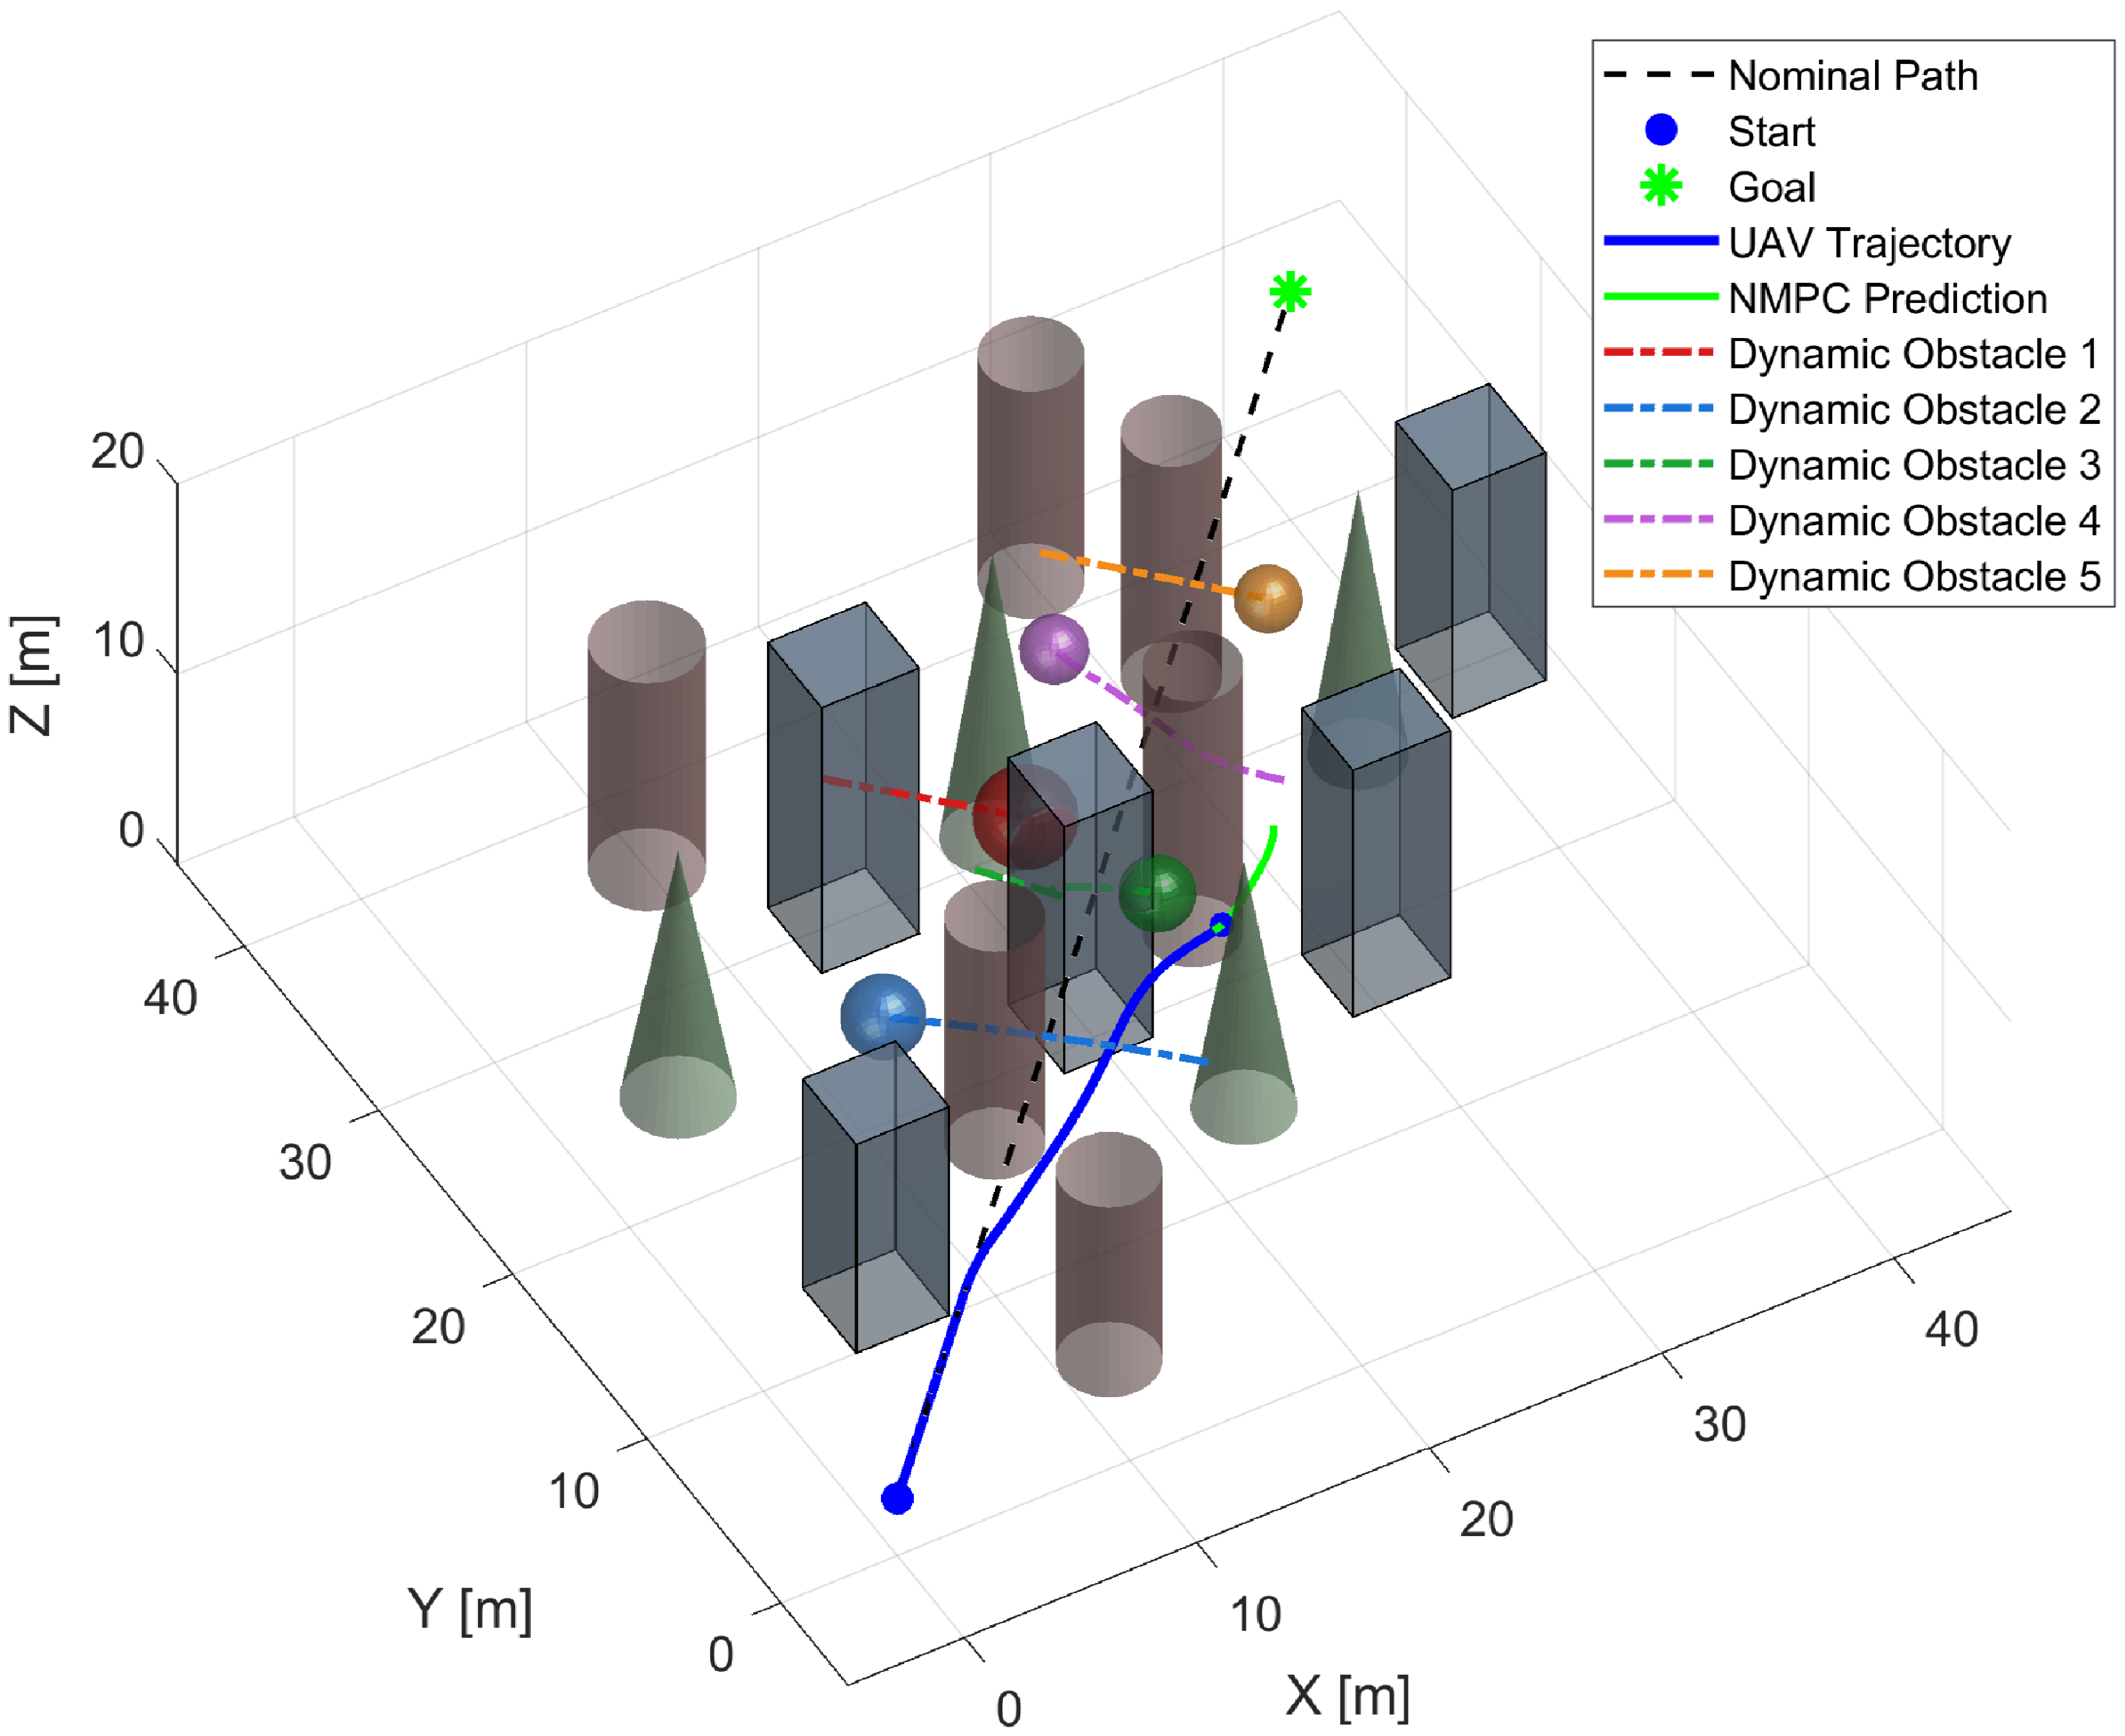
\includegraphics[width=\linewidth]{2} 
		\caption{Snapshot of the dynamic encounter. The UAV starts from the blue marker and moves toward the green goal marker, while multiple dynamic obstacles follow heterogeneous trajectories with different velocities.} 
		\label{fig:snapshot} 
	\end{minipage}%
	\hfill 
	\begin{minipage}{0.32\linewidth} 
		\centering 
		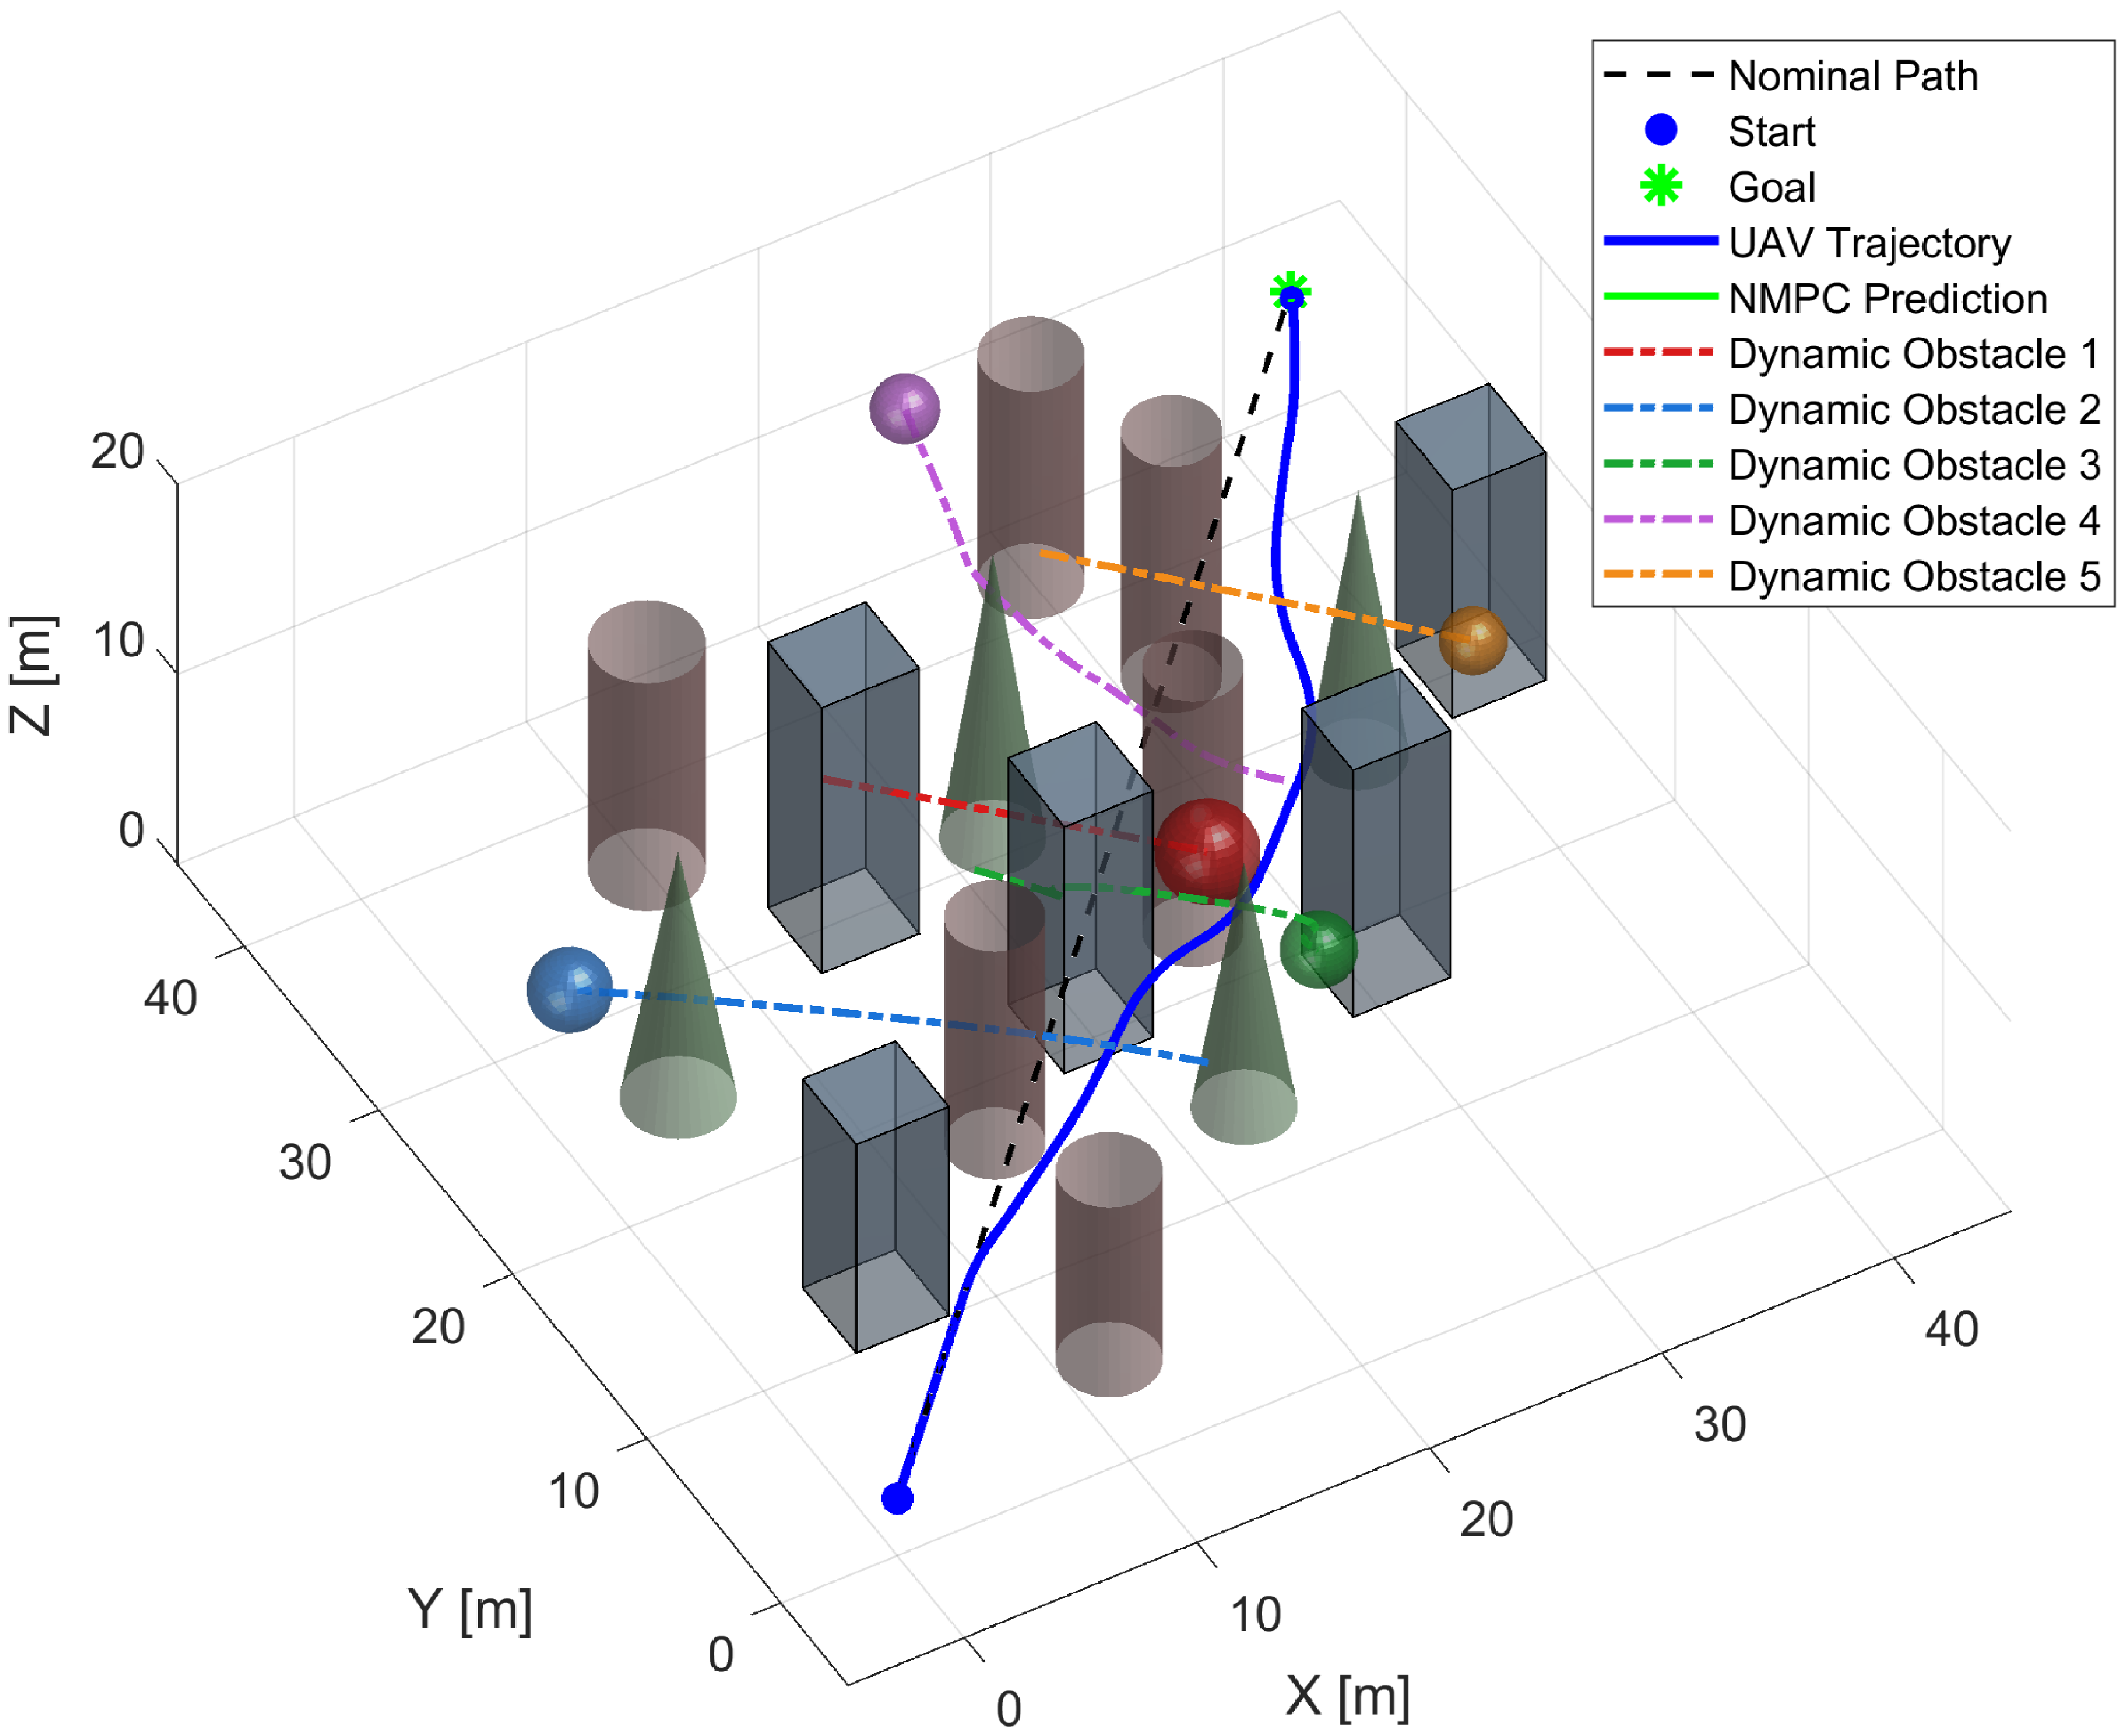
\includegraphics[width=\linewidth]{3} 
		\caption{Complete collision-free UAV trajectory generated by the proposed ET-NMPC under static obstacles and heterogeneous dynamic obstacle motions.} 
		\label{fig:complete} 
	\end{minipage}%
	\hfill 
	\begin{minipage}{0.32\linewidth} 
		\centering 
		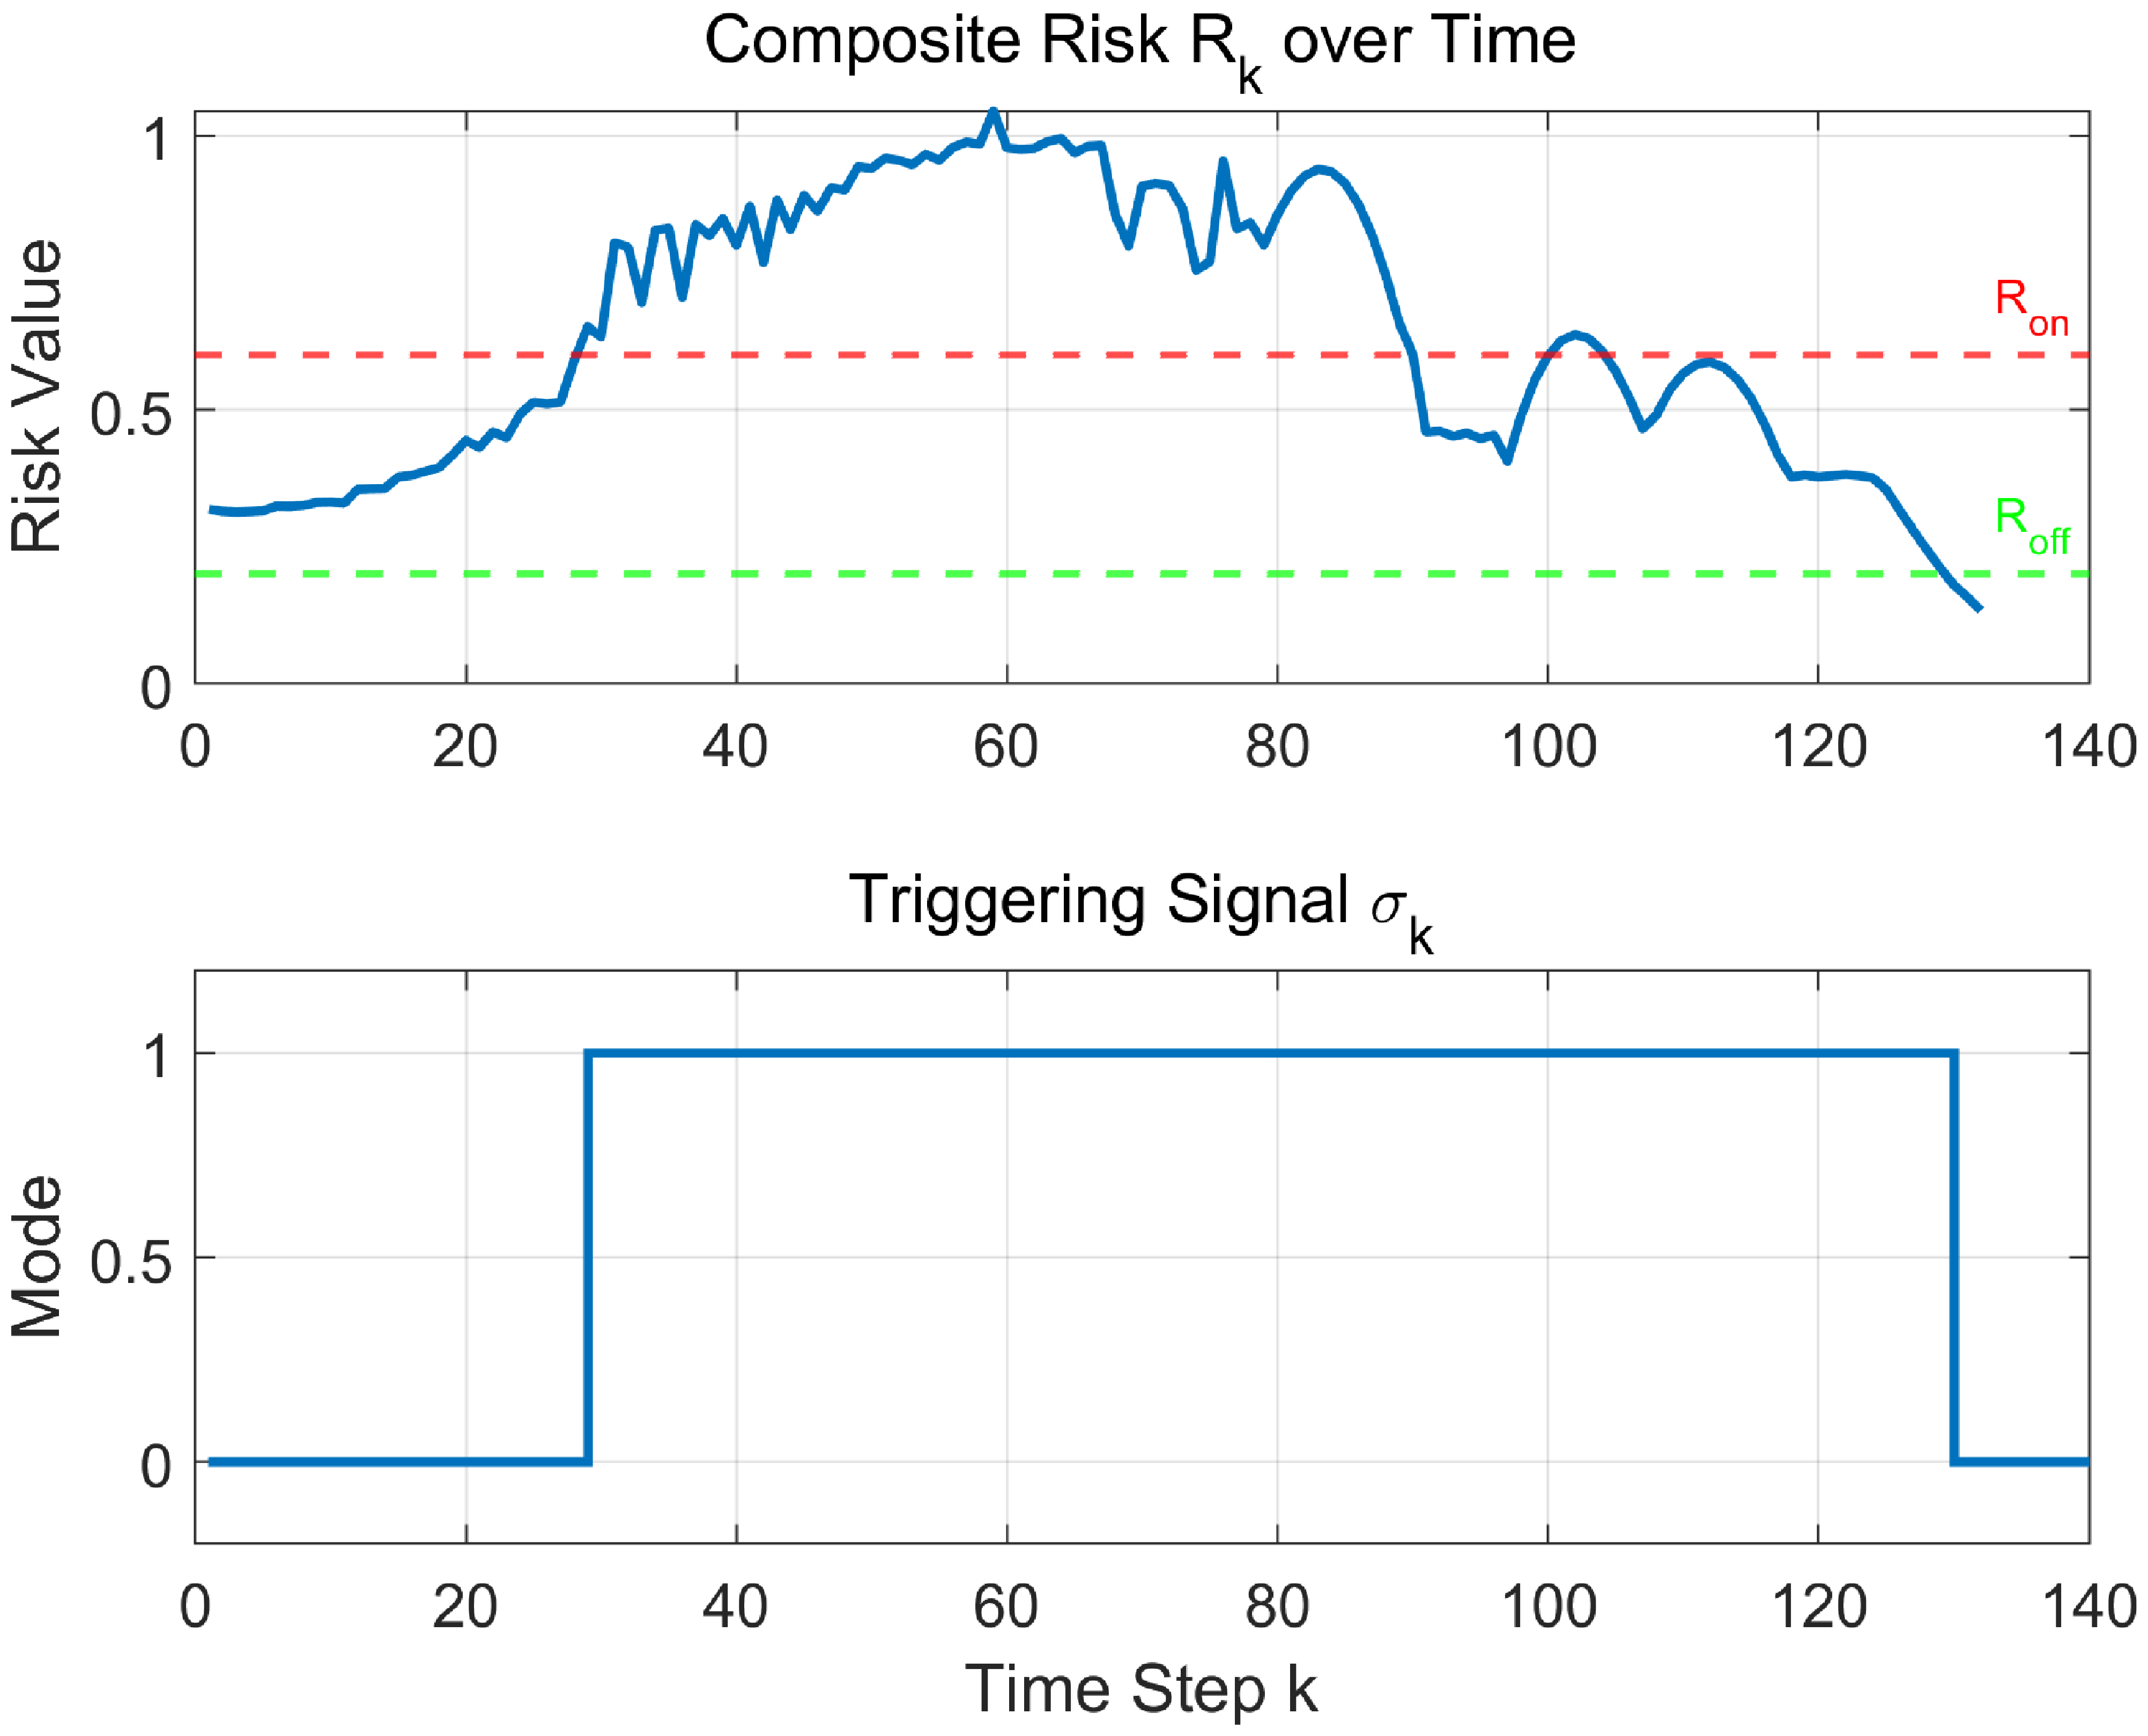
\includegraphics[width=\linewidth]{4} 
		\caption{Composite risk $R_k$ and triggering signal $\sigma_k$. The NMPC solver is activated when $R_k \ge R_{on}$ and deactivated when $R_k \le R_{off}$.} 
		\label{fig:temporal_logic} 
	\end{minipage} 
\end{figure*}

\subsection{Comparative Analysis with Baseline Methods}

To further validate the proposed framework, we compare ET-NMPC with five baseline methods: continuous NMPC (C-NMPC), event-triggered NMPC without prediction (NP-ET-NMPC), event-triggered NMPC with symmetric energy cost (SE-ET-NMPC), 3D artificial potential field (3D-APF)~\cite{ref16}, and Rapidly-exploring Random Tree Star (RRT*). All methods are tested in the same complex urban environment with identical static maps, dynamic obstacle initialization, and random seeds.

\textcolor{blue}{C-NMPC, NP-ET-NMPC, and SE-ET-NMPC serve as internal ablation baselines for examining event-triggered activation, obstacle prediction, and the energy-aware formulation, respectively. 3D-APF and RRT* represent reactive-avoidance and sampling-based-planning paradigms. Thus, the baseline set spans predictive control, event-triggered operation, energy-aware optimization, reactive planning, and sampling-based planning. All algorithms are compared under identical initial conditions, static maps, dynamic-obstacle realizations, and random seeds. The NMPC-based variants share the same system model, prediction horizon, constraints, and solver settings. All methods use the same available obstacle observations, while only the prediction-based NMPC variants exploit future obstacle-state estimation within their original formulations. RRT* is executed in closed loop through periodic replanning with updated obstacle states and collision checking during execution. Recent prediction-based avoidance methods mainly address motion prediction and trajectory generation; they are complementary to, rather than directly equivalent to, the present focus on resource-aware online control and adaptive NMPC activation.}

\textcolor{blue}{Table~\ref{tab:baseline_comparison} reports the quantitative results over 30 randomized trials. The proposed ET-NMPC achieves a 100.0\% success rate, which is the highest among all methods. Compared with C-NMPC, it reduces the trigger rate from 100.0\% to 77.7\% and reduces the average CPU time from 2588.46 ms to 2163.62 ms. It also decreases the control effort from 119.83 to 107.92 while maintaining a comparable estimated energy proxy of 0.8082 Wh. Although NP-ET-NMPC obtains lower CPU time and a lower model-based energy proxy, its success rate drops to 83.3\%, and its clearance decreases to 1.44 m. Therefore, the proposed ET-NMPC achieves an overall trade-off among reliability, safety, computational efficiency, and energy-aware performance; the isolated influence of the asymmetric climb penalty is evaluated by the paired ablation in Table~\ref{tab:asymmetric_climb_ablation}.}

\textcolor{blue}{All baseline comparisons are conducted using 30 paired randomized trials, where identical initial conditions, static maps, dynamic-obstacle trajectories, and random seeds are shared among all algorithms. The continuous results in Table~\ref{tab:baseline_comparison} are reported as mean $\pm$ standard deviation over successful trials. For each trial, all methods receive the same obstacle observations, while only the prediction-based NMPC variants additionally exploit future obstacle-state estimation within their original formulations.}

\textcolor{blue}{For the 29 paired trials with valid continuous metrics, the CPU-time difference (C-NMPC minus ET-NMPC) was 425.11 ms (95\% CI: [372.62, 477.60] ms), confirming the reliability of the reported computational improvement. The paired differences in minimum clearance (ET-NMPC minus C-NMPC) and control effort (C-NMPC minus ET-NMPC) were 0.009 m (95\% CI: [-0.076, 0.094] m) and 11.83 (95\% CI: [10.82, 12.84]), respectively.}

Fig.~\ref{fig:baseline_comparison} shows the trajectory comparison. The proposed ET-NMPC generates a smooth and collision-free trajectory by using dynamic obstacle prediction and risk-triggered local replanning. This predictive information helps the UAV respond before the dynamic obstacle reaches the nominal path. In contrast, 3D-APF becomes trapped by local minima, and \textcolor{blue}{RRT* shows limited performance under dynamic obstacle motion because it does not explicitly optimize future obstacle interactions during closed-loop execution.} \textcolor{blue}{NP-ET-NMPC has lower computation time and a lower model-based energy proxy in some cases, but it has a smaller clearance and a lower success rate.} This result shows that prediction is important for safe dynamic obstacle avoidance.

\begin{table*}[t]
	\centering
	\caption{Quantitative Performance Comparison of Different Algorithms in a Complex Dynamic Urban Scenario}
	\label{tab:baseline_comparison}
	\scriptsize
	\setlength{\tabcolsep}{1.5pt}
	\renewcommand{\arraystretch}{1.25} 
	\begin{tabular*}{\textwidth}{@{\extracolsep{\fill}}lccccccc}
		\toprule[1.1pt]
		\textbf{Algorithm} & \textbf{Success (\%)} & \textbf{Trigger (\%)} & \textbf{Avg CPU (ms)} & \textbf{Clearance (m)} & \textbf{Effort} & \textbf{Climb (m)} & \textcolor{blue}{\textbf{Est. energy proxy (Wh)}} \\
		\midrule
		\textbf{Proposed ET-NMPC} & \textcolor{blue}{100.0 (30/30)} & \textcolor{blue}{77.7 $\pm$ 1.4} & \textcolor{blue}{2163.62 $\pm$ 70.39} & \textcolor{blue}{1.94 $\pm$ 0.67} & \textcolor{blue}{107.92 $\pm$ 5.10} & \textcolor{blue}{11.59 $\pm$ 1.17} & \textcolor{blue}{0.8082 $\pm$ 0.0336} \\
		C-NMPC & \textcolor{blue}{96.7 (29/30)} & \textcolor{blue}{100.0 $\pm$ 0.0} & \textcolor{blue}{2588.46 $\pm$ 136.94} & \textcolor{blue}{1.95 $\pm$ 0.63} & \textcolor{blue}{119.83 $\pm$ 5.36} & \textcolor{blue}{11.67 $\pm$ 1.32} & \textcolor{blue}{0.8199 $\pm$ 0.0389} \\
		NP-ET-NMPC & \textcolor{blue}{83.3 (25/30)} & \textcolor{blue}{75.0 $\pm$ 0.4} & \textcolor{blue}{1862.95 $\pm$ 11.26} & \textcolor{blue}{1.44 $\pm$ 0.86} & \textcolor{blue}{103.56 $\pm$ 1.47} & \textcolor{blue}{10.97 $\pm$ 0.38} & \textcolor{blue}{0.7944 $\pm$ 0.0078} \\
		SE-ET-NMPC & \textcolor{blue}{96.7 (29/30)} & \textcolor{blue}{77.7 $\pm$ 1.4} & \textcolor{blue}{1918.71 $\pm$ 35.32} & \textcolor{blue}{1.96 $\pm$ 0.67} & \textcolor{blue}{107.65 $\pm$ 4.85} & \textcolor{blue}{11.46 $\pm$ 1.17} & \textcolor{blue}{0.8047 $\pm$ 0.0310} \\
		3D-APF & \textcolor{blue}{13.3 (4/30)} & \textcolor{blue}{0.0 $\pm$ 0.0} & \textcolor{blue}{0.13 $\pm$ 0.12} & \textcolor{blue}{0.54 $\pm$ 0.43} & \textcolor{blue}{132.03 $\pm$ 15.67} & \textcolor{blue}{11.17 $\pm$ 1.34} & \textcolor{blue}{0.9548 $\pm$ 0.1449} \\
		RRT* & \textcolor{blue}{0.0 (0/30)} & \textcolor{blue}{--} & \textcolor{blue}{--} & \textcolor{blue}{--} & \textcolor{blue}{--} & \textcolor{blue}{--} & \textcolor{blue}{--} \\
		\bottomrule[1.1pt]
	\end{tabular*}
	\smallskip
	\begin{minipage}{\textwidth}
		\footnotesize
		\textcolor{blue}{\textit{Note: Success is reported as rate (successful trials/30). Collision counts for Proposed ET-NMPC, C-NMPC, NP-ET-NMPC, SE-ET-NMPC, 3D-APF, and RRT* are 0/30, 1/30, 5/30, 1/30, 26/30, and 30/30, respectively. Continuous metrics are reported as mean $\pm$ standard deviation over successful trials. For failed trials, only success and collision statistics are counted.}}
	\end{minipage}
\end{table*}

\begin{figure}[htbp] 
	\centering 
	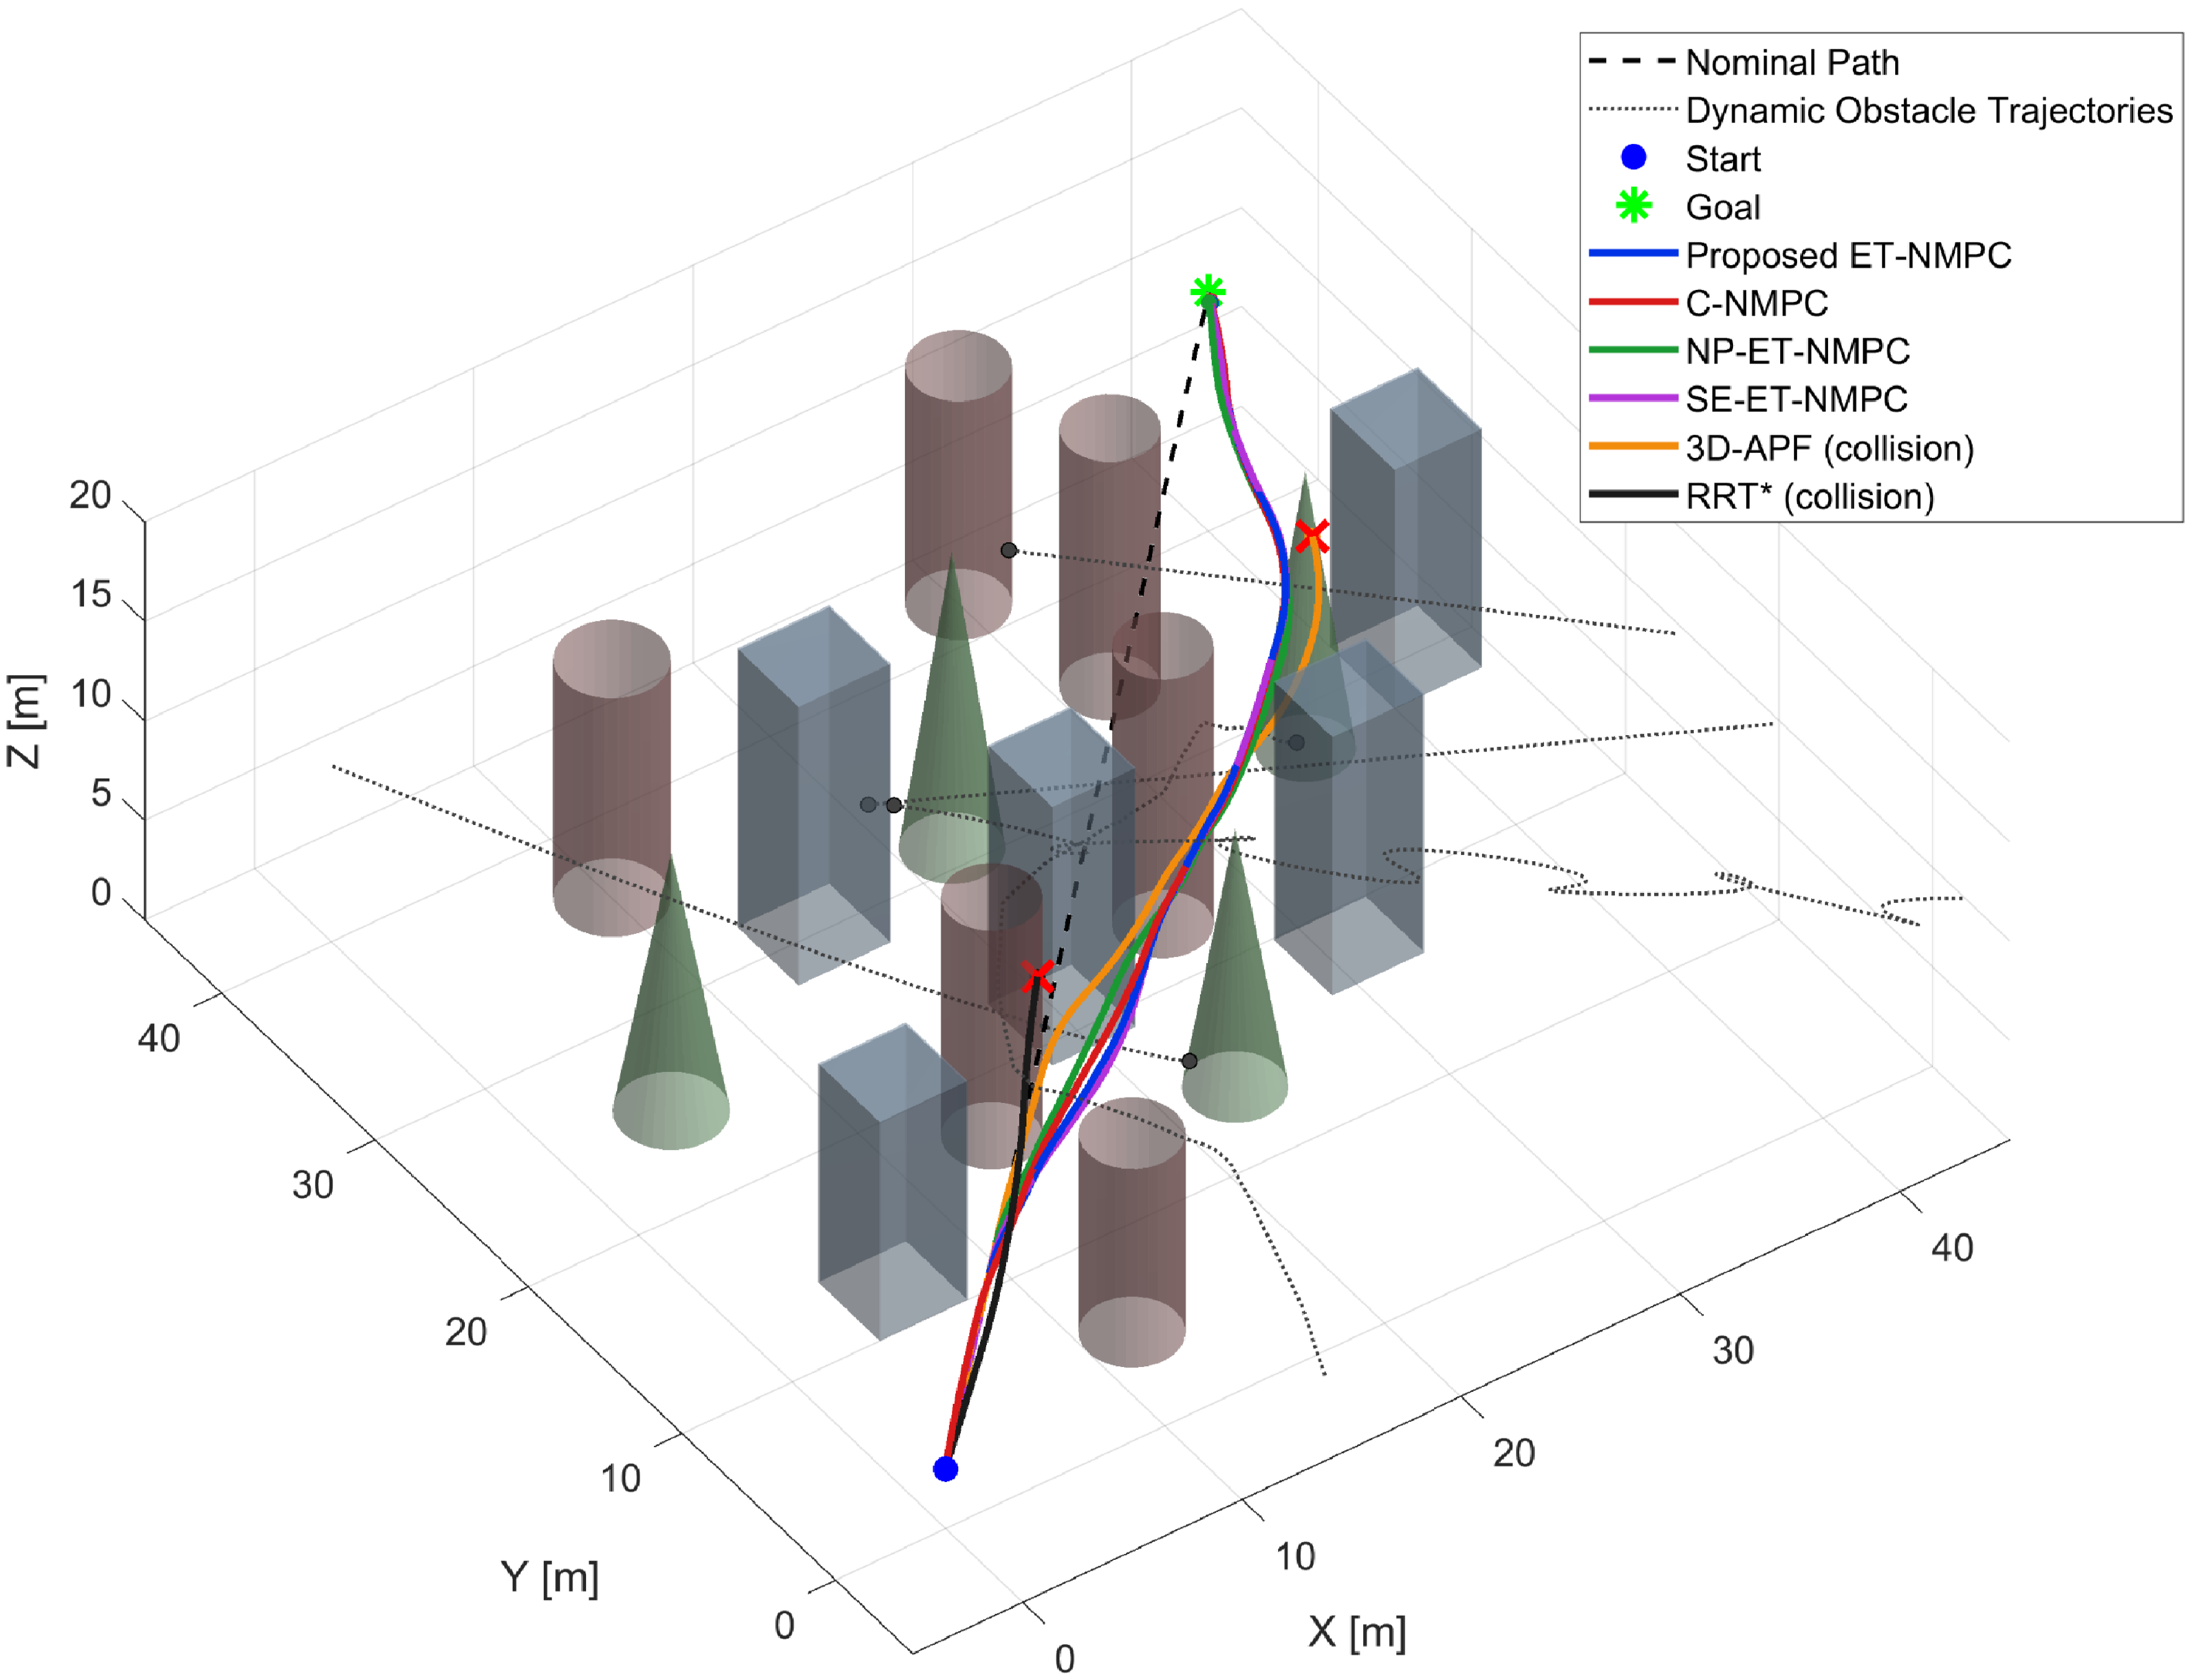
\includegraphics[width=0.90\columnwidth, trim={1cm 1cm 1cm 1cm}, clip]{5} 
	\caption{Trajectory comparison of different path-planning algorithms under the same UAV initial condition, goal position, static map, and dynamic obstacle trajectories.} 
	\label{fig:baseline_comparison} 
\end{figure}

\subsection{\textcolor{blue}{Paired Ablation of the Asymmetric Climb Penalty}}

\textcolor{blue}{To isolate the influence of the asymmetric climb penalty, we conducted 30 paired Monte Carlo scenarios comparing Asymmetric ET-NMPC with Symmetric-energy ET-NMPC. For each paired scenario, both controllers used the same random seed, static map, UAV initial state, goal position, dynamic-obstacle realization, and measurement-noise sequence. The only changed setting was the additional positive-climb penalty: the asymmetric controller used $c_3=3.0$, whereas the symmetric-energy controller disabled this term by setting $c_3=0$.}

\begin{table*}[t]
	\centering
	\caption{\textcolor{blue}{Paired Ablation Results for the Asymmetric Climb Penalty over 30 Matched Scenarios}}
	\label{tab:asymmetric_climb_ablation}
	\footnotesize
	\renewcommand{\arraystretch}{1.15}
	\setlength{\tabcolsep}{2.5pt}
	\resizebox{\textwidth}{!}{%
		\begin{tabular}{l c c c c c c c c c}
			\toprule
			\textcolor{blue}{\textbf{Algorithm}} & \textcolor{blue}{\textbf{Success (\%)}} & \textcolor{blue}{\textbf{Collision (\%)}} & \textcolor{blue}{\textbf{Total positive climb (m)}} & \textcolor{blue}{\textbf{Estimated energy proxy (Wh)}} & \textcolor{blue}{\textbf{Path length (m)}} & \textcolor{blue}{\textbf{Flight time (s)}} & \textcolor{blue}{\textbf{Minimum clearance (m)}} & \textcolor{blue}{\textbf{Trigger rate (\%)}} & \textcolor{blue}{\textbf{Control effort}} \\
			\midrule
			\textcolor{blue}{Asymmetric ET-NMPC} & \textcolor{blue}{100.0} & \textcolor{blue}{0.0} & \textcolor{blue}{11.52 $\pm$ 1.20} & \textcolor{blue}{0.22554 $\pm$ 0.01187} & \textcolor{blue}{60.55 $\pm$ 1.43} & \textcolor{blue}{13.55 $\pm$ 0.58} & \textcolor{blue}{1.93 $\pm$ 0.66} & \textcolor{blue}{77.92 $\pm$ 1.45} & \textcolor{blue}{107.51 $\pm$ 5.43} \\
			\textcolor{blue}{Symmetric-energy ET-NMPC} & \textcolor{blue}{96.7} & \textcolor{blue}{3.3} & \textcolor{blue}{11.30 $\pm$ 1.23} & \textcolor{blue}{0.22186 $\pm$ 0.01807} & \textcolor{blue}{59.67 $\pm$ 4.60} & \textcolor{blue}{13.34 $\pm$ 1.09} & \textcolor{blue}{1.93 $\pm$ 0.66} & \textcolor{blue}{77.45 $\pm$ 2.69} & \textcolor{blue}{105.83 $\pm$ 9.60} \\
			\bottomrule
		\end{tabular}%
	}
	\vspace{2pt}
	\begin{flushleft}
		\textcolor{blue}{\textit{Note: Continuous metrics are reported as mean $\pm$ standard deviation over 30 trials. Paired differences are defined as Asymmetric $-$ Symmetric. Estimated energy is a model-based mission-energy proxy rather than a hardware battery measurement.}}
	\end{flushleft}
\end{table*}

\textcolor{blue}{The asymmetric controller achieved 30/30 successful trials with no collision, whereas the symmetric-energy controller achieved 29/30 successful trials with one collision. The paired difference in total positive climb was 0.217 m (95\% CI: [$-0.069$, $0.503$]), and the paired difference in estimated energy proxy was 0.00368 Wh (95\% CI: [$-0.00169$, $0.00904$]), where each difference is defined as Asymmetric $-$ Symmetric. Both confidence intervals include zero. Therefore, this experiment does not provide statistical evidence that the asymmetric penalty reduces cumulative positive climb or estimated mission energy under the tested parameterization. Instead, the additional term shapes altitude-related optimization preference and provides energy-aware altitude regulation within the safety--energy tradeoff.}

\subsection{Robustness and Parameter Sensitivity Analysis}

To further evaluate the robustness of the proposed ET-NMPC framework, we conduct a parameter sensitivity analysis in the complex dynamic urban scenario. The experiment includes five dynamic obstacles with heterogeneous motion trajectories, including constant-velocity, constant-acceleration, sinusoidal, and random maneuvering motions. Measurement noise is also added to the obstacle observations. This setting introduces model mismatch between the lightweight online prediction model and the actual obstacle motion, and therefore provides a more challenging test for the proposed risk-triggered predictive control framework.

\begin{figure}[htbp]
	\centering
	% 第一行：图(a)和图(b)
	\begin{minipage}{0.48\linewidth}
		\centering
		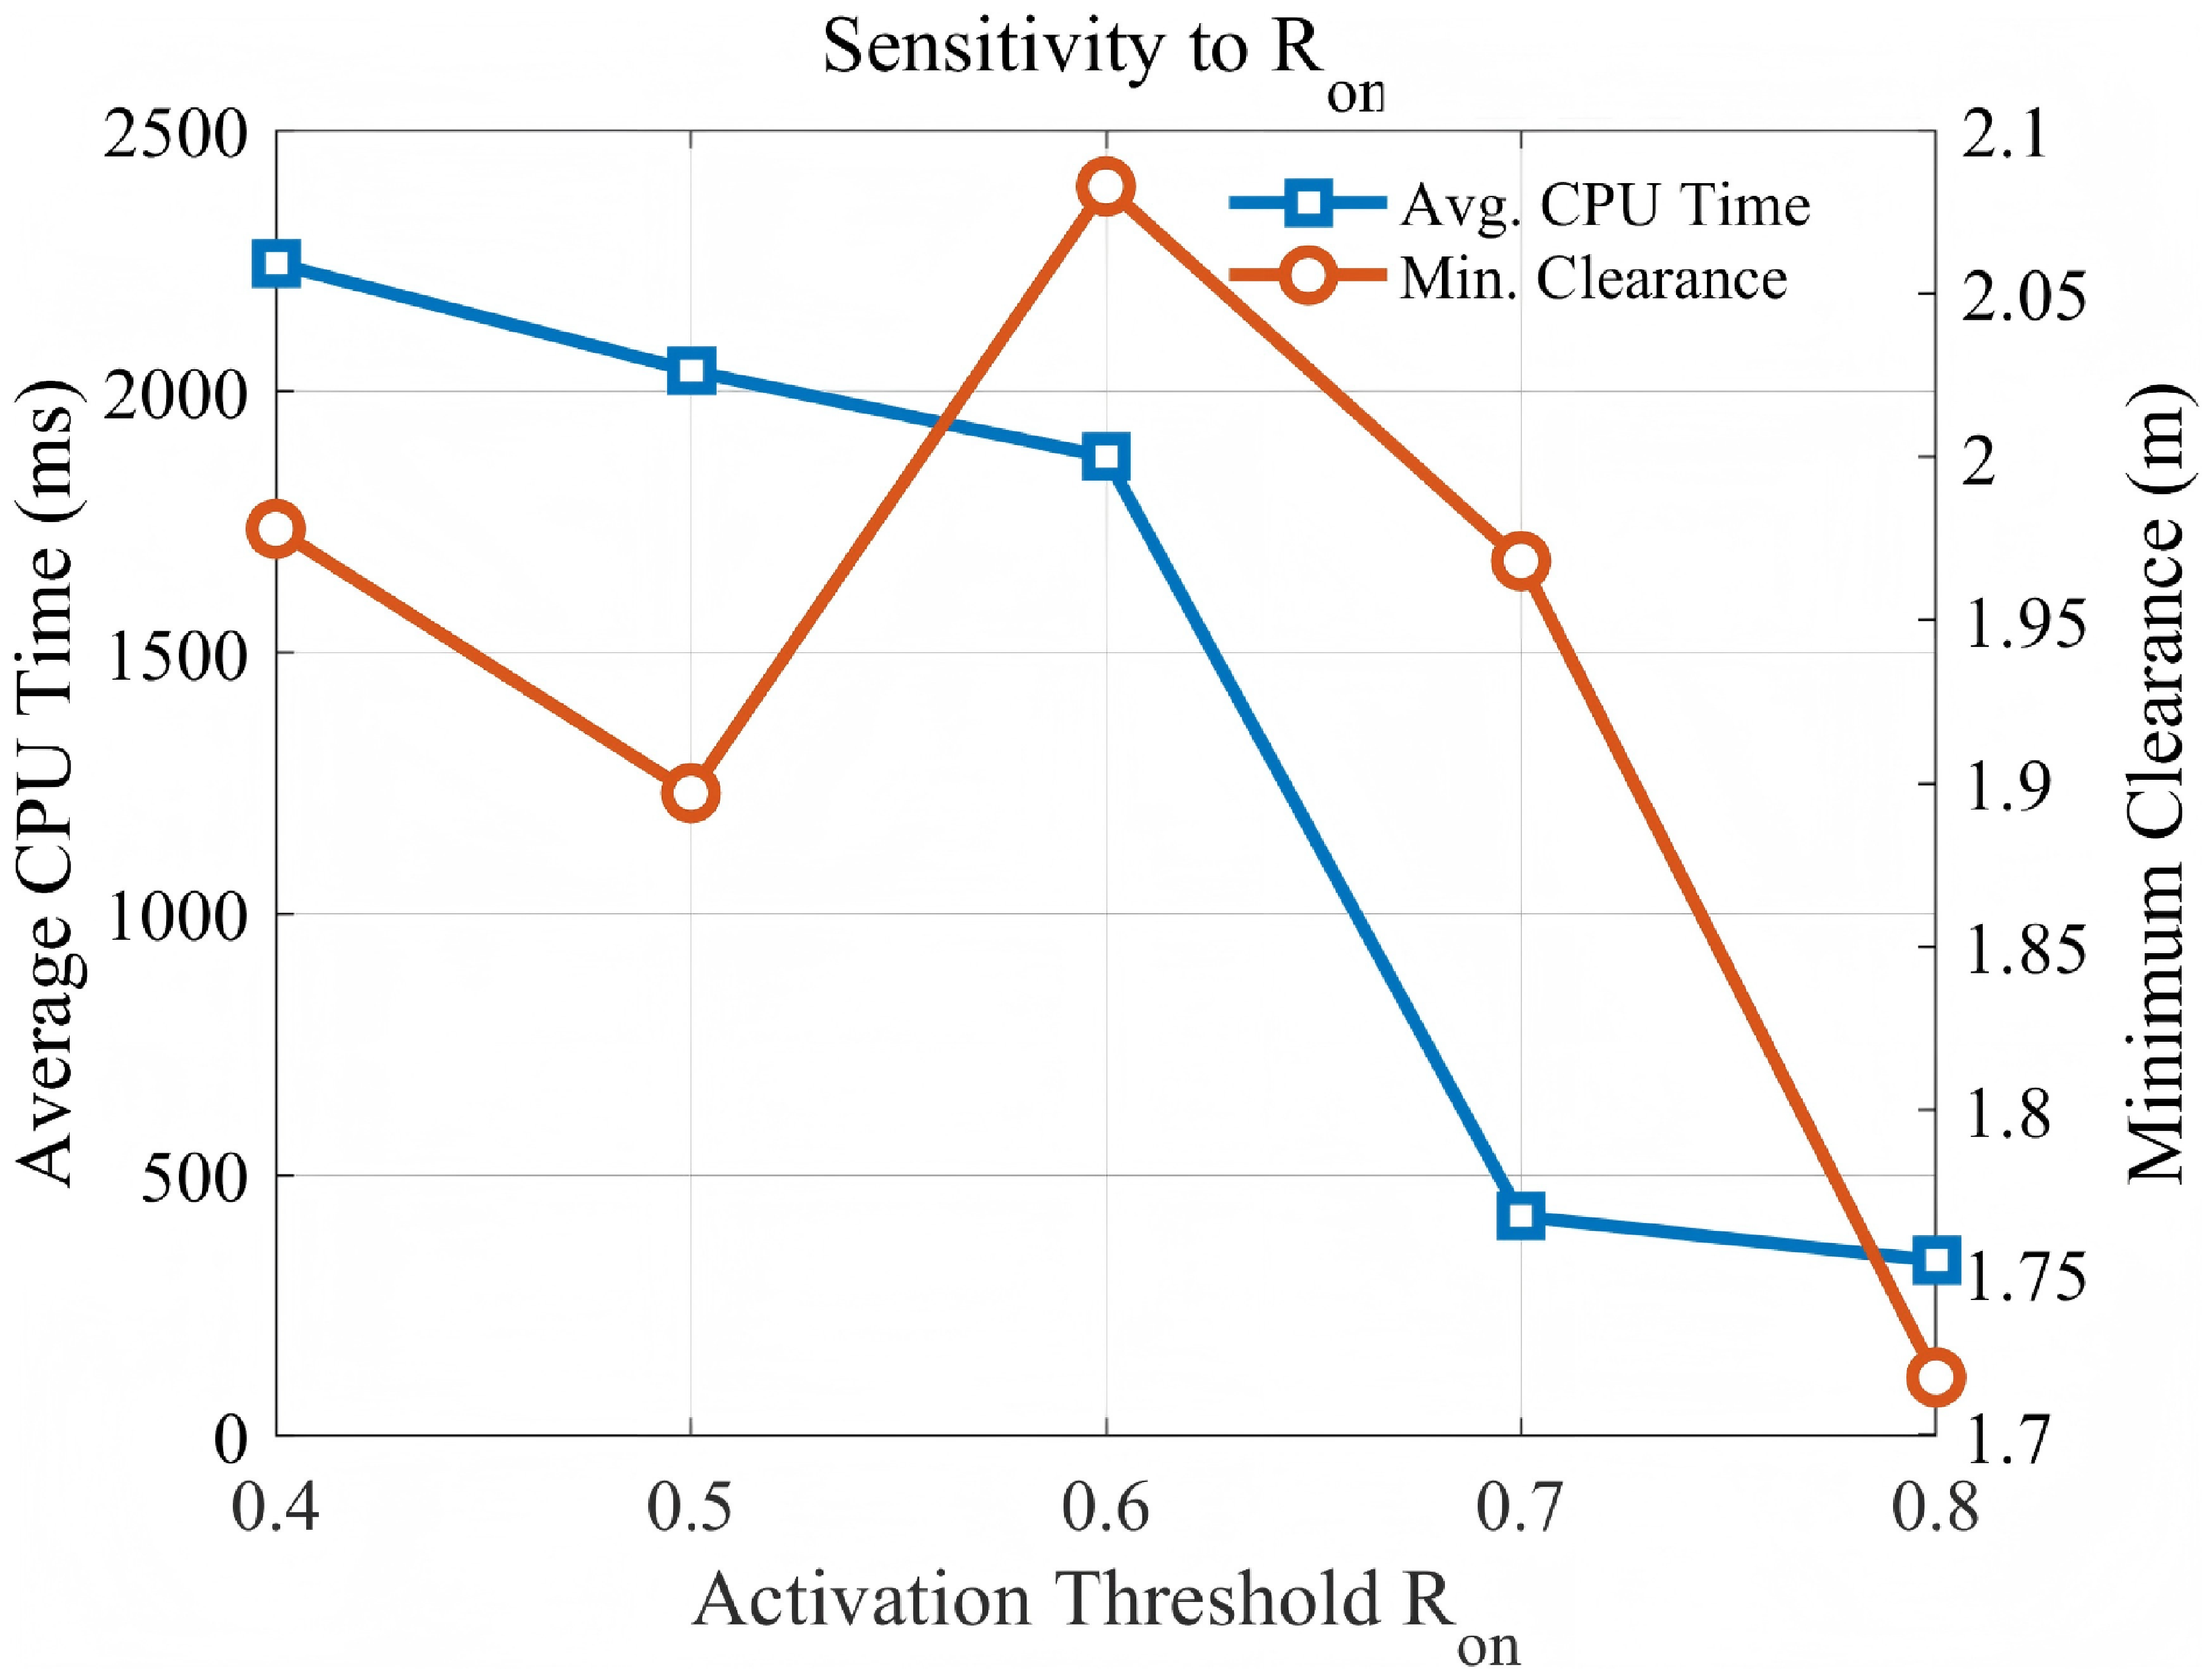
\includegraphics[width=\linewidth, trim={0.1cm 0.1cm 0.1cm 0.1cm}, clip]{6}
		\vspace{-2pt}
		{\small (a)}
	\end{minipage}%
	\hfill
	\begin{minipage}{0.48\linewidth}
		\centering
		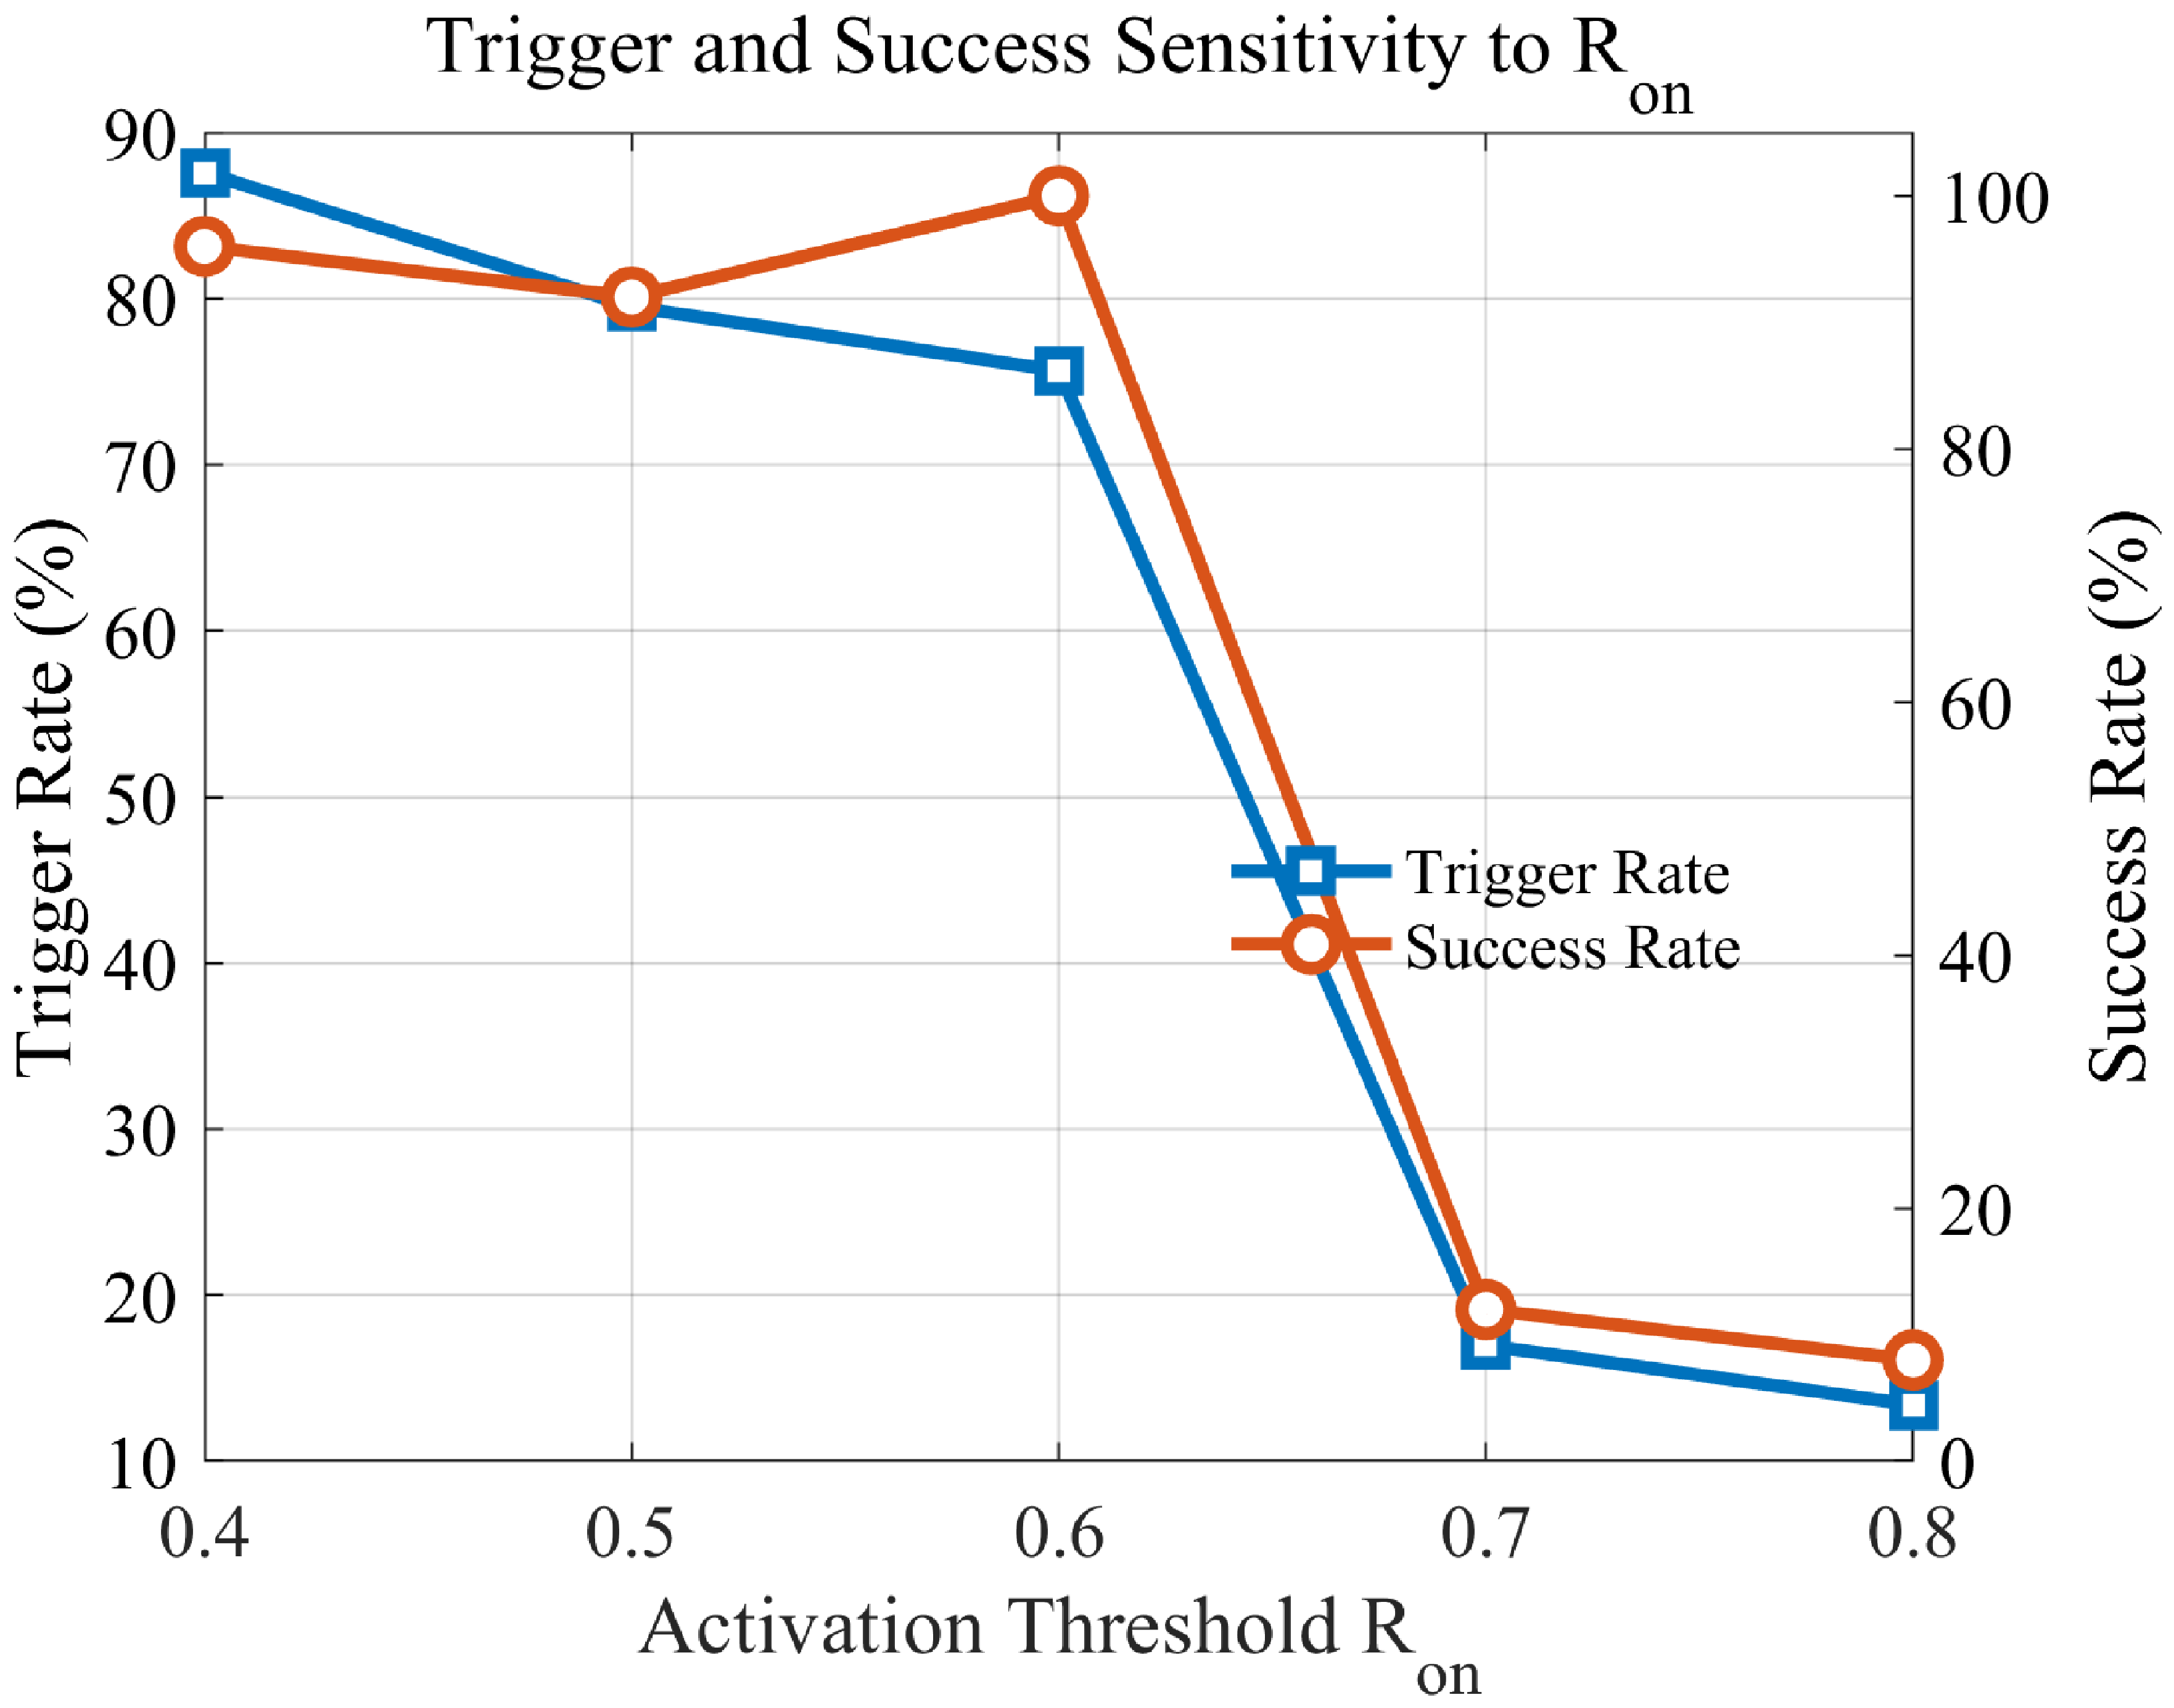
\includegraphics[width=\linewidth, trim={0.1cm 0.1cm 0.1cm 0.1cm}, clip]{7}
		\vspace{-2pt}
		{\small (b)}
	\end{minipage}
	
	\vspace{4pt}
	% 第二行：图(c)和图(d)
	\begin{minipage}{0.48\linewidth}
		\centering
		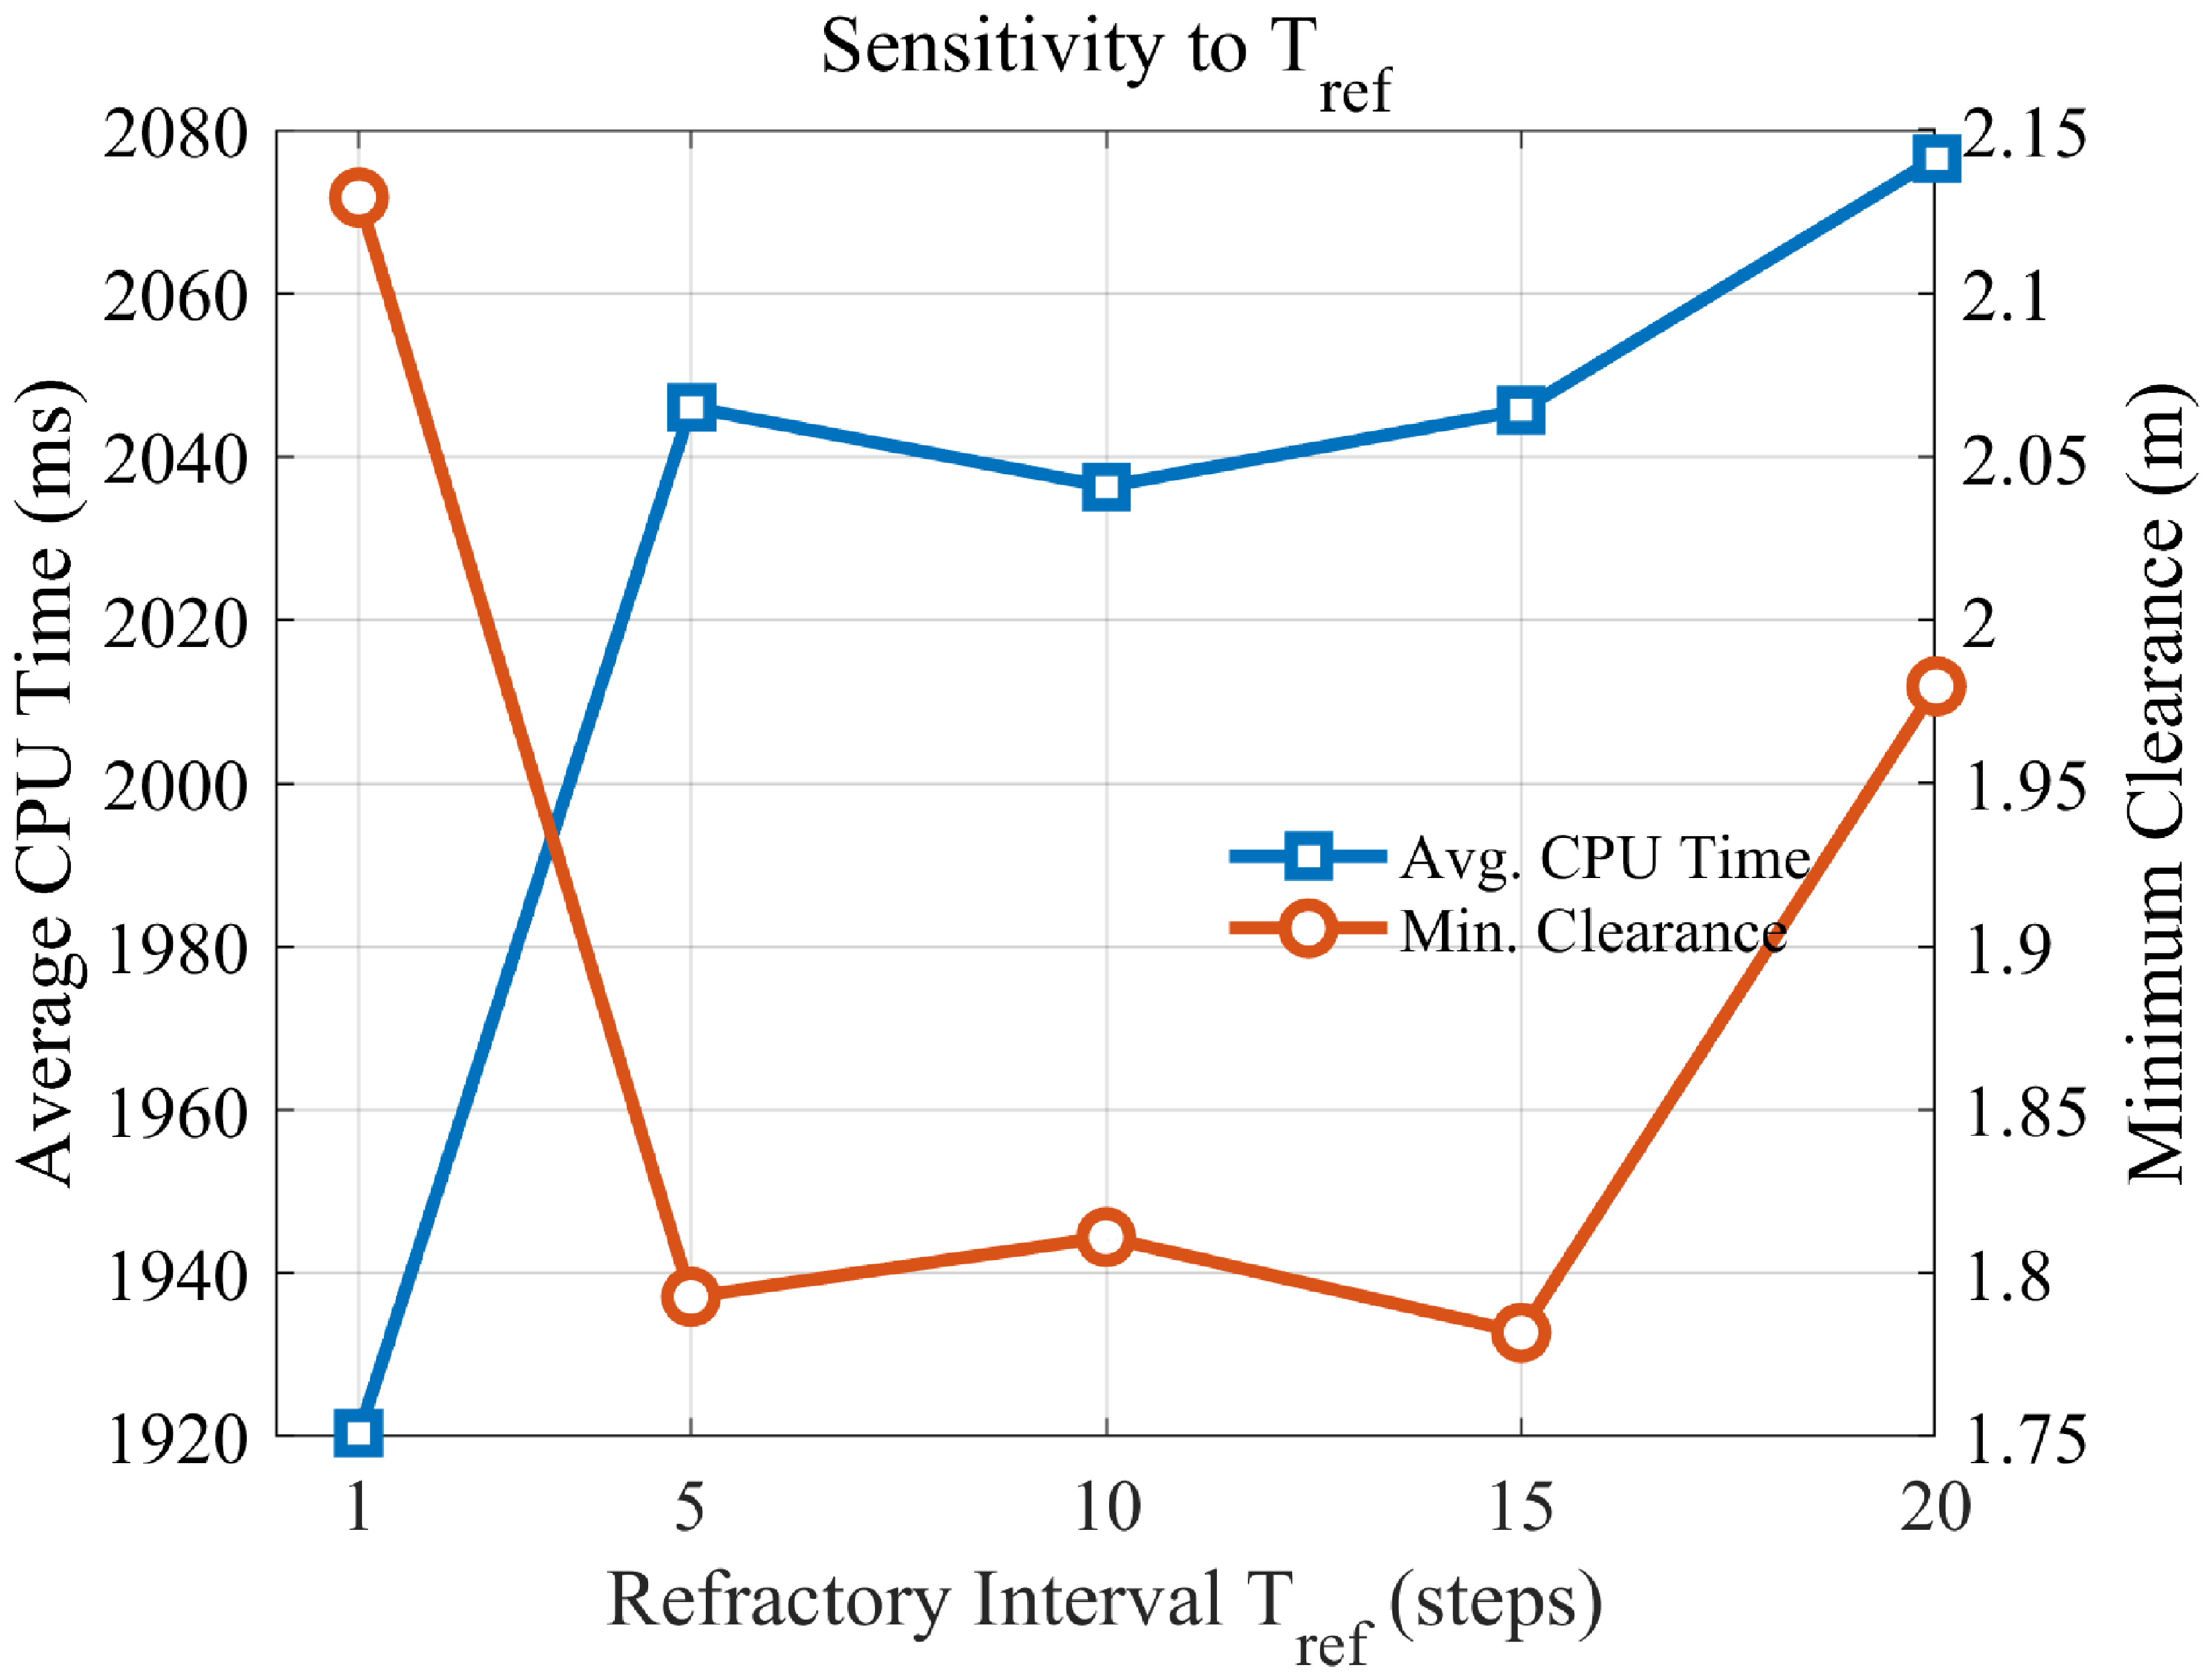
\includegraphics[width=\linewidth, trim={0.1cm 0.1cm 0.1cm 0.1cm}, clip]{8}
		\vspace{-2pt}
		{\small (c)}
	\end{minipage}%
	\hfill
	\begin{minipage}{0.48\linewidth}
		\centering
		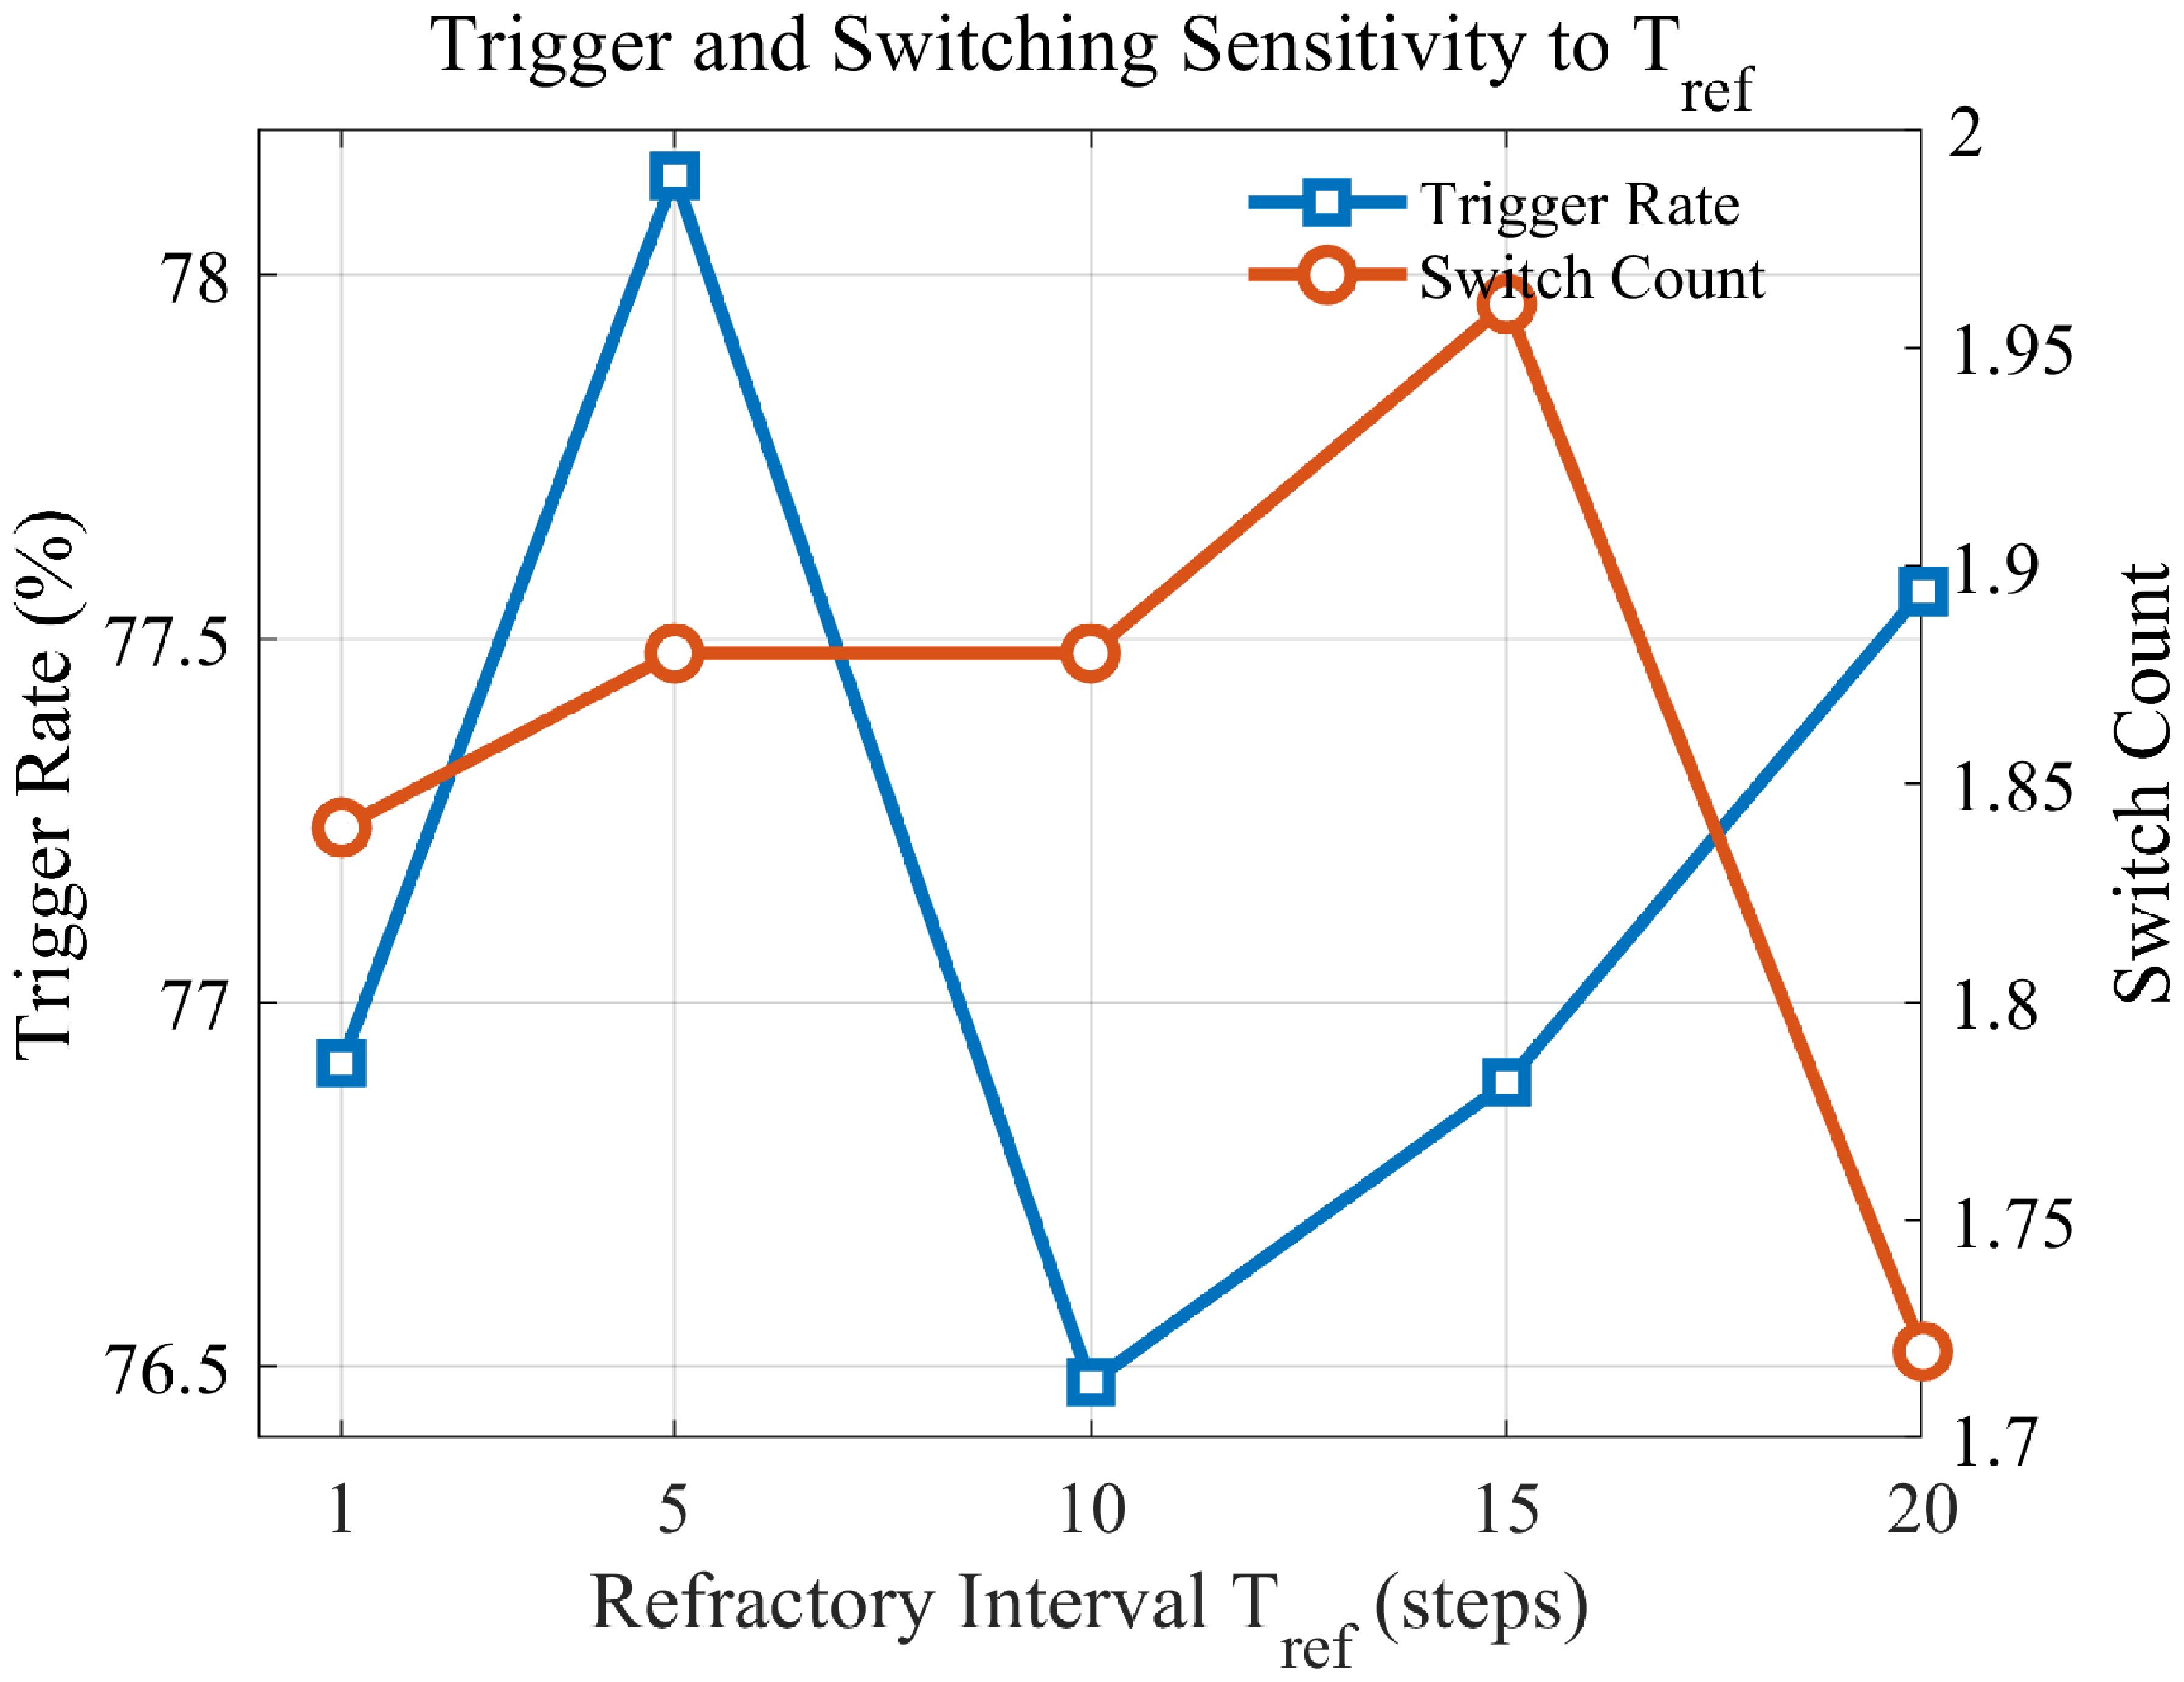
\includegraphics[width=\linewidth, trim={0.1cm 0.1cm 0.1cm 0.1cm}, clip]{9}
		\vspace{-2pt}
		{\small (d)}
	\end{minipage}
	
	\caption{Robustness and parameter sensitivity analysis under heterogeneous dynamic obstacle motions and measurement noise. 
		(a) CPU time and minimum clearance versus the risk activation threshold $R_{on}$. 
		(b) Trigger rate and success rate versus $R_{on}$. 
		(c) CPU time and minimum clearance versus the refractory interval $T_{ref}$. 
		(d) Trigger rate and switch count versus $T_{ref}$.}
	\label{fig:sensitivity_analysis}
\end{figure}

For each parameter setting, 30 independent randomized trials are conducted. We evaluate two event-triggering parameters, namely the risk activation threshold $R_{on}$ and the refractory interval $T_{ref}$. Fig.~\ref{fig:sensitivity_analysis} shows the sensitivity results. As shown in Fig.~\ref{fig:sensitivity_analysis}(a) and Fig.~\ref{fig:sensitivity_analysis}(b), $R_{on}$ affects the trade-off between computational efficiency and avoidance reliability. When $R_{on}$ is 0.4 or 0.5, the controller triggers more often, which increases the trigger rate and CPU time. When $R_{on}$ increases to 0.7 or 0.8, the trigger rate decreases, but the success rate also drops. This result shows that a large activation threshold may delay replanning under fast-changing obstacle motion. In contrast, $R_{on}=0.6$ achieves a 100.0\% success rate, an average CPU time of 1874.83 ms, and the largest minimum clearance of 2.08 m. Therefore, $R_{on}=0.6$ is selected in this work.

Fig.~\ref{fig:sensitivity_analysis}(c) and Fig.~\ref{fig:sensitivity_analysis}(d) show the influence of $T_{ref}$. The trigger rate changes only slightly over the tested values, and the switch count remains low. This result shows that the hysteresis-based logic can suppress frequent mode switching. Among the tested values, $T_{ref}=5$ achieves a 100.0\% success rate with acceptable CPU time. Therefore, $T_{ref}=5$ is used in the following experiments.

The weighting coefficients in Table~\ref{tab:key_parameters} are selected by empirical tuning under safety, smoothness, and energy-awareness requirements. The risk-related weights give priority to collision avoidance in high-risk regions. The tracking and control-effort weights maintain smooth motion and bounded acceleration. \textcolor{blue}{The asymmetric climb and energy-related weights regulate the tradeoff between altitude motion and energy-related cost. These weights are fixed in all reported experiments; their isolated influence is evaluated by the paired ablation, which does not claim statistically significant reduction in cumulative positive climb or estimated mission energy.} However, fixed weights may be sub-optimal under different operating conditions. Future work will study adaptive weighting mechanisms for more diverse environments.

\subsection{\textcolor{blue}{Computational Performance Profiling and Deadline-Oriented Analysis}}

To disclose the computational performance of the proposed method, we conducted a profiling experiment before the Monte Carlo evaluation. Table~\ref{tab:computational_profiling} reports the timing distribution, IPOPT iterations, solver settings, memory usage, and triggering status. The results show that the event-triggered strategy avoids solving the NMPC problem at every sampling instant. Non-triggered steps require almost negligible computation, while the main cost comes from triggered NMPC optimization. This supports the computational advantage of the proposed risk-triggered scheduling mechanism. \textcolor{blue}{The reported computation time measures the controller computation process in MATLAB/CasADi simulation, including the triggered NMPC solving procedure, rather than the complete physical closed-loop latency including communication and hardware execution.}

\begin{table}[h]
	\centering
	\caption{\textcolor{blue}{Deadline-oriented computational statistics and solver disclosure of the proposed ET-NMPC.}}
	\label{tab:computational_profiling}
	\scriptsize
	\setlength{\tabcolsep}{2.5pt}
	\renewcommand{\arraystretch}{1.12}
	\begin{tabular}{p{0.46\columnwidth}p{0.46\columnwidth}}
		\toprule
		\textbf{Item} & \textbf{Value} \\
		\midrule
		\multicolumn{2}{l}{\textbf{Profiling setup}} \\
		Number of profiling runs & 30 \\
		Total simulation steps & 4072 \\
		Number of dynamic obstacles & 5 \\
		Triggered steps & 3183 \\
		Trigger rate & $77.8 \pm 3.5\%$ \\
		\midrule
		\multicolumn{2}{l}{\textbf{IPOPT statistics}} \\
		Average IPOPT iterations & $22.0 \pm 12.9$ \\
		Maximum IPOPT iterations & 87 \\
		Solver failure count & 0 \\
		Fallback count & 0 \\
		\midrule
		\multicolumn{2}{l}{\textbf{Memory statistics}} \\
		Mean memory before simulation & 6361.1 MB \\
		Mean memory after simulation & 6356.9 MB \\
		Mean memory variation & -4.2 MB \\
		Peak observed memory & 6367.6 MB \\
		\midrule
		\multicolumn{2}{l}{\textbf{Solver settings}} \\
		IPOPT maximum iterations & 100 \\
		IPOPT tolerance & $10^{-4}$ \\
		IPOPT acceptable tolerance & $10^{-3}$ \\
		Sparse linear solver & MUMPS \\
		Warm-start strategy & Shifted reference initialization \\
		\bottomrule
	\end{tabular}

	\medskip
	\textcolor{blue}{\textbf{Deadline-oriented timing statistics (pooled step-level values)}}\\
	\resizebox{\columnwidth}{!}{%
		\begin{tabular}{lccccc}
			\toprule
			\textcolor{blue}{\textbf{Metric}} & \textcolor{blue}{\textbf{Mean (ms)}} & \textcolor{blue}{\textbf{Median (ms)}} & \textcolor{blue}{\textbf{95th percentile (ms)}} & \textcolor{blue}{\textbf{99th percentile (ms)}} & \textcolor{blue}{\textbf{Maximum (ms)}} \\
			\midrule
			\textcolor{blue}{All controller steps} & \textcolor{blue}{2077.9} & \textcolor{blue}{2551.9} & \textcolor{blue}{2964.7} & \textcolor{blue}{3150.4} & \textcolor{blue}{3982.8} \\
			\textcolor{blue}{Triggered NMPC steps} & \textcolor{blue}{2658.3} & \textcolor{blue}{2596.2} & \textcolor{blue}{2987.2} & \textcolor{blue}{3187.8} & \textcolor{blue}{3982.8} \\
			\midrule
			\textcolor{blue}{Deadline} & \multicolumn{5}{c}{\textcolor{blue}{100 ms ($\Delta t=0.1$ s)}} \\
			\textcolor{blue}{Violation ratio (all steps)} & \multicolumn{5}{c}{\textcolor{blue}{3183/4072 (78.168\%)}} \\
			\textcolor{blue}{Violation ratio (triggered steps)} & \multicolumn{5}{c}{\textcolor{blue}{3183/3183 (100.0\%)}} \\
			\bottomrule
		\end{tabular}%
	}
\end{table}

\textcolor{blue}{Table~\ref{tab:computational_profiling} also reports the IPOPT statistics and solver configuration for the reported desktop MATLAB/CasADi implementation. The average IPOPT iteration number remains below the maximum iteration limit, and no solver failure or fallback occurs during the profiling runs. The profiling configuration uses IPOPT with the MUMPS sparse linear solver, fixed convergence tolerances, and shifted-reference warm start. The memory values refer to the MATLAB process during the reported runs; they indicate no continuous process-memory growth in this desktop experiment, but they are not solver-specific or embedded-memory measurements.}

\textcolor{blue}{Although the event-triggered strategy significantly reduces unnecessary NMPC calls, the current desktop MATLAB/CasADi implementation does not satisfy the strict 100-ms deadline for triggered optimization steps. With $\Delta t=0.1$ s, the deadline-violation ratio is 78.168\% over all recorded controller steps and 100.0\% over the triggered NMPC steps. Therefore, the reported results characterize desktop computational behavior and relative computational savings rather than hard real-time or onboard feasibility. Future validation on embedded platforms, hardware-in-the-loop experiments, and compiled implementations will be considered in future work.}

\begin{table*}[t!]
	\centering
	\caption{Monte Carlo Performance under Different Numbers of Dynamic Obstacles}
	\label{tab:monte_carlo_scalability}
	\footnotesize
	\renewcommand{\arraystretch}{1.15}
	\setlength{\tabcolsep}{3pt}
	\resizebox{\textwidth}{!}{%
		\begin{tabular}{c l c c c c c c}
			\toprule
			\textbf{Obstacles} & \textbf{Algorithm} & \textbf{Success (\%)} & \textbf{Trigger (\%)} & \textbf{Avg CPU (ms)} & \textbf{CPU Saving (\%)} & \textbf{Clearance (m)} & \textbf{Est. Energy (Wh)} \\
			\midrule
			\multirow{4}{*}{1}
			& \textbf{Proposed ET-NMPC} & \textbf{100.0} & 75.4 $\pm$ 0.4 & 1818.92 $\pm$ 21.52 & 24.2 & 5.11 $\pm$ 1.35 & 0.2179 $\pm$ 0.0021 \\
			& C-NMPC & 100.0 & 100.0 $\pm$ 0.0 & 2398.80 $\pm$ 10.04 & 0.0 & 5.08 $\pm$ 1.38 & 0.2187 $\pm$ 0.0028 \\
			& NP-ET-NMPC & 100.0 & 74.7 $\pm$ 0.2 & 1804.73 $\pm$ 13.96 & 24.8 & 5.22 $\pm$ 1.72 & 0.2189 $\pm$ 0.0009 \\
			& SE-ET-NMPC & 100.0 & 75.4 $\pm$ 0.4 & 1819.68 $\pm$ 54.27 & 24.1 & 5.49 $\pm$ 1.52 & 0.2180 $\pm$ 0.0018 \\
			\midrule
			\multirow{4}{*}{3}
			& \textbf{Proposed ET-NMPC} & \textbf{100.0} & 76.3 $\pm$ 1.6 & 1923.78 $\pm$ 41.73 & 24.0 & 2.83 $\pm$ 0.78 & 0.2254 $\pm$ 0.0091 \\
			& C-NMPC & 99.0 & 100.0 $\pm$ 0.0 & 2531.26 $\pm$ 35.28 & 0.0 & 2.71 $\pm$ 0.82 & 0.2245 $\pm$ 0.0082 \\
			& NP-ET-NMPC & 95.0 & 75.1 $\pm$ 0.4 & 1905.06 $\pm$ 28.33 & 24.7 & 2.25 $\pm$ 0.98 & 0.2197 $\pm$ 0.0013 \\
			& SE-ET-NMPC & 99.0 & 76.4 $\pm$ 1.0 & 1915.05 $\pm$ 25.87 & 24.3 & 2.77 $\pm$ 0.78 & 0.2235 $\pm$ 0.0079 \\
			\midrule
			\multirow{4}{*}{5}
			& \textbf{Proposed ET-NMPC} & \textbf{100.0} & 78.3 $\pm$ 1.4 & 2074.76 $\pm$ 38.70 & 21.1 & 2.05 $\pm$ 0.62 & 0.2298 $\pm$ 0.0129 \\
			& C-NMPC & 97.0 & 100.0 $\pm$ 0.0 & 2628.69 $\pm$ 21.45 & 0.0 & 1.88 $\pm$ 0.60 & 0.2271 $\pm$ 0.0116 \\
			& NP-ET-NMPC & 90.0 & 75.2 $\pm$ 0.7 & 1917.88 $\pm$ 49.68 & 27.0 & 1.32 $\pm$ 0.77 & 0.2205 $\pm$ 0.0061 \\
			& SE-ET-NMPC & 97.0 & 78.1 $\pm$ 1.3 & 1933.10 $\pm$ 34.46 & 26.5 & 1.86 $\pm$ 0.57 & 0.2286 $\pm$ 0.0155 \\
			\bottomrule
		\end{tabular}%
	}
	\vspace{2pt}
	\footnotesize
	\begin{flushleft}
		\textit{Note: Continuous metrics are reported as mean $\pm$ 95\% confidence interval over 100 independent runs. CPU saving is computed relative to C-NMPC under the same number of dynamic obstacles.}
	\end{flushleft}
\end{table*}

\subsection{Quantitative Monte Carlo Stress Test}

To evaluate the robustness and scalability of the proposed framework under uncertainty, Monte Carlo stress tests are conducted under different numbers of dynamic obstacles. The number of dynamic obstacles is set to 1, 3, and 5. For each obstacle setting, 100 independent randomized trials are performed. Gaussian noise is added to the obstacle measurements, and the initial states of the dynamic obstacles are randomly perturbed. The statistical results are reported in Table~\ref{tab:monte_carlo_scalability}.

The results show that the proposed ET-NMPC maintains a 100.0\% success rate in all tested scenarios. This result indicates that the proposed method can preserve robust obstacle avoidance when the dynamic obstacle density increases. In contrast, the performance of the baseline methods degrades as the number of dynamic obstacles increases. When the number of dynamic obstacles is 5, the success rates of C-NMPC, NP-ET-NMPC, and SE-ET-NMPC decrease to 97.0\%, 90.0\%, and 97.0\%, respectively. The no-prediction variant NP-ET-NMPC shows the most obvious degradation, which confirms the importance of predictive obstacle motion estimation in complex dynamic environments.

The proposed ET-NMPC also achieves a clear computational advantage over the continuous C-NMPC baseline. Since C-NMPC solves the NMPC problem at every time step, its trigger rate remains 100.0\% in all scenarios. In comparison, the proposed ET-NMPC keeps the trigger rate between 75.4\% and 78.3\%. As a result, it reduces the average CPU time by 24.2\%, 24.0\%, and 21.1\% for 1, 3, and 5 dynamic obstacles, respectively. This result supports the computational benefit of the risk-triggered scheduling mechanism.

The safety margin also supports the advantage of the proposed method. When the number of dynamic obstacles increases to 5, the proposed ET-NMPC achieves the largest clearance of 2.05 m. This value is higher than those of C-NMPC, NP-ET-NMPC, and SE-ET-NMPC. Although NP-ET-NMPC obtains larger CPU savings in some cases, its success rate and clearance decrease significantly under dense dynamic obstacles. \textcolor{blue}{The estimated energy proxy of the proposed ET-NMPC remains comparable to the other NMPC-based methods. Therefore, these obstacle-count experiments characterize the overall robustness, safety margin, computational efficiency, and model-based energy-related behavior of the proposed framework; they do not isolate a statistically significant energy reduction attributable to the asymmetric climb penalty.}

\section{Conclusion}

This paper proposed an energy-aware event-triggered NMPC framework for UAV obstacle avoidance in complex 3D dynamic environments. The framework uses a composite risk index to schedule the NMPC solver. It also uses receding-horizon prediction to estimate dynamic obstacle motion. The UAV follows nominal tracking in low-risk states. The NMPC solver generates a local collision-free trajectory in high-risk states. This dual-mode strategy reduces unnecessary optimization calls and preserves motion safety.

\textcolor{blue}{From an IoT-system perspective, the proposed method provides a resource-aware local perception--control component for a mobile sensing-and-actuation node, with the demonstrated benefit of avoiding unnecessary NMPC activations and associated local computational workload.}

Simulation results verified the effectiveness of the proposed method. Comparative experiments showed that the proposed ET-NMPC achieves a good balance among safety, computational efficiency, and energy-aware performance. The prediction mechanism improves avoidance performance under dynamic threats. \textcolor{blue}{The asymmetric climb penalty introduces an energy-aware altitude regulation mechanism by assigning additional cost to positive altitude gains. The paired ablation experiment evaluates its isolated influence without claiming statistically significant reduction in cumulative positive climb or estimated mission energy.} Monte Carlo tests with statistical variations showed robust performance under noise and random obstacle states. \textcolor{blue}{Computational profiling also reported IPOPT iterations, solver settings, MATLAB process-memory observations, and timing distributions. These results characterize desktop computational behavior and relative CPU savings; they do not establish hard real-time operation at the 0.1-s deadline or embedded feasibility.}

\textcolor{blue}{Future work will consider validation on embedded platforms, hardware-in-the-loop experiments, and compiled implementations, together with prediction enhancement and theoretical extension. We will extend the constant-velocity prediction model to more nonlinear and uncertain obstacle motions, study adaptive weighting mechanisms and terminal-set-based stability analysis, and investigate cooperative multi-UAV obstacle avoidance in real cluttered environments.}


\begin{thebibliography}{35}
	\bibliographystyle{IEEEtran}
	
	\bibitem{ref1} R. Li and B. Xin, ``Autonomous navigation of quadrotors in dynamic complex environments,'' \textit{IEEE Trans. Ind. Electron.}, vol. 72, no. 3, pp. 2790--2800, 2024.
	\bibitem{ref2} Y. Zeng and R. Zhang, ``Energy-efficient UAV communication with trajectory optimization,'' \textit{IEEE Trans. Wireless Commun.}, vol. 16, no. 6, pp. 3747--3760, 2017.
	\bibitem{ref3} B. Lindqvist, S. S. Mansouri, A. A. Agha-mohammadi, and G. Nikolakopoulos, ``Nonlinear MPC for collision avoidance and control of UAVs with dynamic obstacles,'' \textit{IEEE Robot. Autom. Lett.}, vol. 5, no. 4, pp. 6001--6008, 2020.
	\bibitem{ref4} G. Chen, W. Dong, P. Peng, J. Alonso-Mora, and X. Zhu, ``Continuous occupancy mapping in dynamic environments using particles,'' \textit{IEEE Trans. Robot.}, vol. 40, pp. 64--84, 2023.
	\bibitem{ref5} G. Chen, S. Wu, M. Shi, W. Dong, H. Zhu, and J. Alonso-Mora, ``RAST: Risk-aware spatio-temporal safety corridors for MAV navigation in dynamic uncertain environments,'' \textit{IEEE Robot. Autom. Lett.}, vol. 8, no. 2, pp. 808--815, 2022.
	\bibitem{ref6} E. Xu, C. Yu, and Y. Liu, ``Topological risk-based path selection in dynamic environments,'' in \textit{Proc. IEEE 18th Int. Conf. Control Autom. (ICCA)}, 2024, pp. 767--772.
	\bibitem{ref7} B. Pang, X. Hu, W. Dai, and K. H. Low, ``UAV path optimization with an integrated cost assessment model considering third-party risks in metropolitan environments,'' \textit{Reliab. Eng. Syst. Saf.}, vol. 222, pp. 108399, 2022.
	\bibitem{ref8} J. Yu, Y. Xu, J. Zhang, K. Cai, and K. K. Ng, ``Risk-aware UAS path planning based on four-dimensional operation volume construction and dynamic collision avoidance,'' in \textit{Proc. AIAA DATC/IEEE 44th Digital Avionics Syst. Conf. (DASC)}, 2025, pp. 1--10.
	\bibitem{ref9} E. Olcay, H. Meeß, and G. Elger, ``Dynamic obstacle avoidance for UAVs using MPC and GP-based motion forecast,'' in \textit{Proc. Eur. Control Conf. (ECC)}, 2024, pp. 1024--1031.
	\bibitem{ref10} Z. Xu, H. Jin, X. Shen, H. Han, and K. Shimada, ``Intent prediction-driven model predictive control for UAV planning and navigation in dynamic environments,'' \textit{IEEE Robot. Autom. Lett.}, vol. 10, no. 5, pp. 4946-4953, 2025.
	\bibitem{ref11} M. Lu, X. Fan, H. Chen, and P. Lu, ``FAPP: Fast and adaptive perception and planning for UAVs in dynamic cluttered environments,'' \textit{IEEE Trans. Robot.}, vol. 41, pp. 871--886, 2024.
	\bibitem{ref12} Z. Wang, Z. Meng, Y. Lin, G. Zhao, J. Wang, and C. Jiang, ``An efficient dynamic obstacle perception and avoidance framework for robust real-time UAV trajectory planning,'' \textit{IEEE Trans. Aerosp. Electron. Syst.}, vol. 61, no. 6, pp. 19412-19426, Dec. 2025.
	\bibitem{ref13} Y. Liang, H. Wang, X. Liu, X. Zhao, Y. Ye, Y. Zheng, and J. Jiang, ``A dynamic obstacle avoidance algorithm for unmanned aerial vehicles based on predictive velocity obstacles,'' \textit{Robot. Auton. Syst.}, vol. 196, pp. 105250, 2026.
	\bibitem{ref14} Y. Zheng, C. Yu, J. Xu, F. Ran, and E. Xu, ``Active perception-planning collaboration for quadrotor dynamic obstacle avoidance with NMPC,'' in \textit{Proc. IEEE Int. Conf. Unmanned Syst. (ICUS)}, 2025, pp. 323--328.
	\bibitem{ref15} D. Wang, J. Wang, S. He, J. Huang, B. Zhang, Y. Wang, and F. Gao, ``Multi-FOV-constrained trajectory planning for multirotor safe landing,'' in \textit{Proc. IEEE/RSJ Int. Conf. Intell. Robots Syst. (IROS)}, 2024, pp. 5356--5363.
	\bibitem{ref16} I. Yadav and H. G. Tanner, ``Reactive receding horizon planning and control for quadrotors with limited on-board sensing,'' in \textit{Proc. IEEE/RSJ Int. Conf. Intell. Robots Syst. (IROS)}, 2020, pp. 7058--7063.
	\bibitem{ref17} D. Jang, C. Y. Son, J. Yoo, H. J. Kim, and K. H. Johansson, ``Efficient networked UAV control using event-triggered predictive control,'' \textit{IFAC-PapersOnLine}, vol. 52, no. 15, pp. 412--417, 2019.
	\bibitem{ref18} D. Du, H. Zhang, Z. Wang, and H. Yan, ``Model predictive formation tracking-containment control for multi-UAVs with obstacle avoidance,'' \textit{IEEE Trans. Syst., Man, Cybern.: Syst.}, vol. 54, no. 6, pp. 3404--3414, Jun. 2024.
	\bibitem{ref19} Y. Wu, M. Chen, H. Li, and M. Chadli, ``Event-triggered-based adaptive NN cooperative control of six-rotor UAVs with finite-time prescribed performance,'' \textit{IEEE Trans. Autom. Sci. Eng.}, vol. 21, no. 2, pp. 1867--1877, 2023.
	\bibitem{ref20} H. Tang and Y. Chen, ``Dynamic event-triggered distributed MPC for UAV-UGV systems against DoS attacks,'' in \textit{Proc. IEEE Int. Conf. Syst. Man Cybern. (SMC)}, pp. 20--25, 2024.
	\bibitem{ref21} S. N. Aspragkathos, G. C. Karras, and K. J. Kyriakopoulos, ``Event-triggered image moments predictive control for tracking evolving features using UAVs,'' \textit{IEEE Robot. Autom. Lett.}, vol. 9, no. 2, pp. 1019--1026, 2023.
	\bibitem{ref22} Y. Ma, H. Yang, J. Zhao, H. Xie, L. Dai, and Y. Xia, ``Cloud-edge cooperative MPC with event-triggered strategy for large-scale complex systems,'' \textit{IEEE Internet Things J.}, vol. 12, no. 15, pp. 31095-31111, Aug. 2025.
	\bibitem{ref23} X. Luo, S. Cen, J. Wang, X. Li, and X. Guan, ``Event-triggered MPC for nonlinear connected autonomous vehicle platoons with a deep reinforcement learning approach,'' \textit{IEEE Trans. Veh. Technol.}, 2026, doi: 10.1109/TVT.2026.3665584. 
	\bibitem{ref24} J. Hu, X. Yang, M. Lou, H. Ye, H. Shen, and Z. Xiang, ``Design, simulation, and field testing of an intelligent control algorithm based on event-triggered and nonlinear MPC for USVs,'' \textit{IEEE Internet Things J.}, vol. 12, no. 12, pp. 22155-22167, 2025.
	\bibitem{ref25} H. Zhang, Y. Wang, and H. Sun, ``Trajectory tracking of unmanned hovercraft: Event-triggered NMPC under actuation limits and disturbances,'' \textit{Actuators}, vol. 15, no. 1, p. 6, 2025.
	\bibitem{ref26} B. Li, Q. Li, Y. Zeng, Y. Rong, and R. Zhang, ``3D trajectory optimization for energy-efficient UAV communication: A control design perspective,'' \textit{IEEE Trans. Wireless Commun.}, vol. 21, no. 6, pp. 4579--4593, 2021.
	\bibitem{ref27} X. Dai, B. Duo, X. Yuan, and M. Di Renzo, ``Energy-efficient UAV communications in the presence of wind: 3D modeling and trajectory design,'' \textit{IEEE Trans. Wireless Commun.}, vol. 23, no. 3, pp. 1840--1854, 2023.
	\bibitem{ref28} L. Zhang, A. Celik, S. Dang, and B. Shihada, ``Energy-efficient trajectory optimization for UAV-assisted IoT networks,'' \textit{IEEE Trans. Mobile Comput.}, vol. 21, no. 12, pp. 4323--4337, 2021.
	\bibitem{ref29} A. H. Arani, M. M. Azari, P. Hu, Y. Zhu, H. Yanikomeroglu, and S. Safavi-Naeini, ``Reinforcement learning for energy-efficient trajectory design of UAVs,'' \textit{IEEE Internet Things J.}, vol. 9, no. 11, pp. 9060--9070, 2021.
	\bibitem{ref30} N. Nouri, J. Abouei, A. R. Sepasian, M. Jaseemuddin, A. Anpalagan, and K. N. Plataniotis, ``Three-dimensional multi-UAV placement and resource allocation for energy-efficient IoT communication,'' \textit{IEEE Internet Things J.}, vol. 9, no. 3, pp. 2134--2152, 2021.
	\bibitem{ref31} H. Gou, S. Zhao, Y. Rao, G. Zhang, J. Sha, Z. Lu, and P. Du, ``Energy-efficient trajectory design and resource allocation for multi-UAV-enabled ISAC in IoT networks,'' \textit{IEEE Trans. Consum. Electron.}, vol. 72, no. 1, pp. 1672-1684, Feb. 2026.
	\bibitem{ref32} X. Zuo, Z. Yang, Y. Fan, R. Yao, J. Xu, and L. Li, ``3D trajectory optimization for energy-efficient UAV communication with obstacle constraints,'' \textit{IEEE Trans. Veh. Technol.}, vol. 75, no. 1, pp. 1073-1084, Jan. 2026.
	\bibitem{ref33} D. Huo, L. Dai, R. Chai, R. Xue, and Y. Xia, ``Collision-free model predictive trajectory tracking control for UAVs in obstacle environment,'' \textit{IEEE Trans. Aerosp. Electron. Syst.}, vol. 59, no. 3, pp. 2920--2932, 2022.
	
\end{thebibliography}

\vfill

\end{document}
